\graphicspath{{Ch2_Experiment/figures/}}

\chapter{The LHC and the ATLAS Detector}

The \textbf{ATLAS} (\textbf{A} \textbf{T}oroidal \textbf{L}HC \textbf{A}pparatu\textbf{S}) is one of four primary detectors constructed to explore the high energy/intensity frontier of modern particle physics by utilizing the \textbf{LHC} (Large Hadron Collider) at the \textbf{CERN} (Conseil Européen pour la Recherche Nucléaire) laboratory in Geneva, Switzerland.

\nomenclature{CERN}{Conseil Européen pour la Recherche Nucléaire}
\nomenclature{LHC}{Large Hadronc Collider}
\nomenclature{ATLAS}{A Toroidal LHC Apparatus}

\section{The Large Hadron Collider}
The LHC is the world's highest energy particle accelerator and the largest machine ever built by humans.
It is composed of over a thousand superconducting magnets, sixteen radio frequency (RF) accelerating cavities, large scale cryogenic systems, and support structures within a circular 27 kilometer subterranean ring.
Its purpose is to accelerate two beams of protons or heavy ions travelling in opposite directions around the ring in ultra-high vacuum (UHV) conditions to 99.9999991\% of the speed of light $(c)$ and collide them into one another at four separate interaction points (IP).

Four large detectors reside at each of these interaction points: ATLAS, CMS (Compact Muon Solenoid), ALICE (A Large Ion Collider Experiment), and LHCb (LHC Beauty).
Vast amounts of data describing the collision products are collected by these detectors and studied by thousands of scientists across the globe.
The ATLAS and CMS detectors are general purpose detectors intended to study the Standard Model, in particular the properties of the Higgs boson, as well as search for new physics beyond the Standard Model (BSM).
The ALICE and LHCb detectors are more specialized, with ALICE focusing on heavy ion collisions to study quark-gluon plasma and LHCb investigating physics involving hadrons containing b-quarks and the matter-antimatter asymmetry of the universe.
The relative positions of these detectors around the ring can be seen in Figure~\ref{fig:cern_accelerator_complex}.

\nomenclature{RF}{\textbf{R}adio \textbf{F}requency}
\nomenclature{IP}{\textbf{I}nteraction \textbf{P}oints where protons collide at the LHC}
\nomenclature{BSM}{\textbf{B}eyond the \textbf{S}tandard \textbf{M}odel}

\subsection{Proton Accelerator Chain}
Before the protons reach the detectors or the LHC ring itself they pass through a chain of prior accelerators as outlined in Figure~\ref{fig:cern_accelerator_complex}.
The protons themselves are obtained from a simple bottle of hydrogen gas.
An electric field is used to strip the hydrogen atoms of their electrons to yield bare protons.
The first accelerator in the chain, LINAC2, accelerates these bare protons up to 50 MeV.
The beam is then injected into the Proton Synchotron Booster (PSB) and accelerated to 1.4 GeV, followed by the Proton Synchotron (PS) itself which accelerates the beam to 25 GeV.

Starting with the PSB the protons begin to assemble into ``bunches'' of $1.15 \times 10^{11}$ protons each as they synchronize with the RF cavity acceleration frequency. 
As the protons pass through the PS acceleration stage, the bunching is modified several times and ultimately results in a time separation between bunches of 25 ns.
In the final step before arriving at the LHC, the protons are accelerated by the Super Proton Synchotron (SPS) up to 450 GeV.
A variety of filling schemes were used by the LHC during stable data-taking periods during Run 2, where the number of bunches per injection varied from 48 to 144, with a maximum of 2556 bunches recorded in the ring at once.
It takes 4 minutes and 20 seconds to fill each of the two LHC beam pipes and an additional 20 minutes to accelerate the protons to their maximum energy of 6.5 TeV for Run 2.
This results in a center-of-mass energy of $\sqrt{s} = 2 \times 6.5\ \mathrm{TeV} = 13\ \mathrm{TeV}$.

\begin{figure}
	\centering
	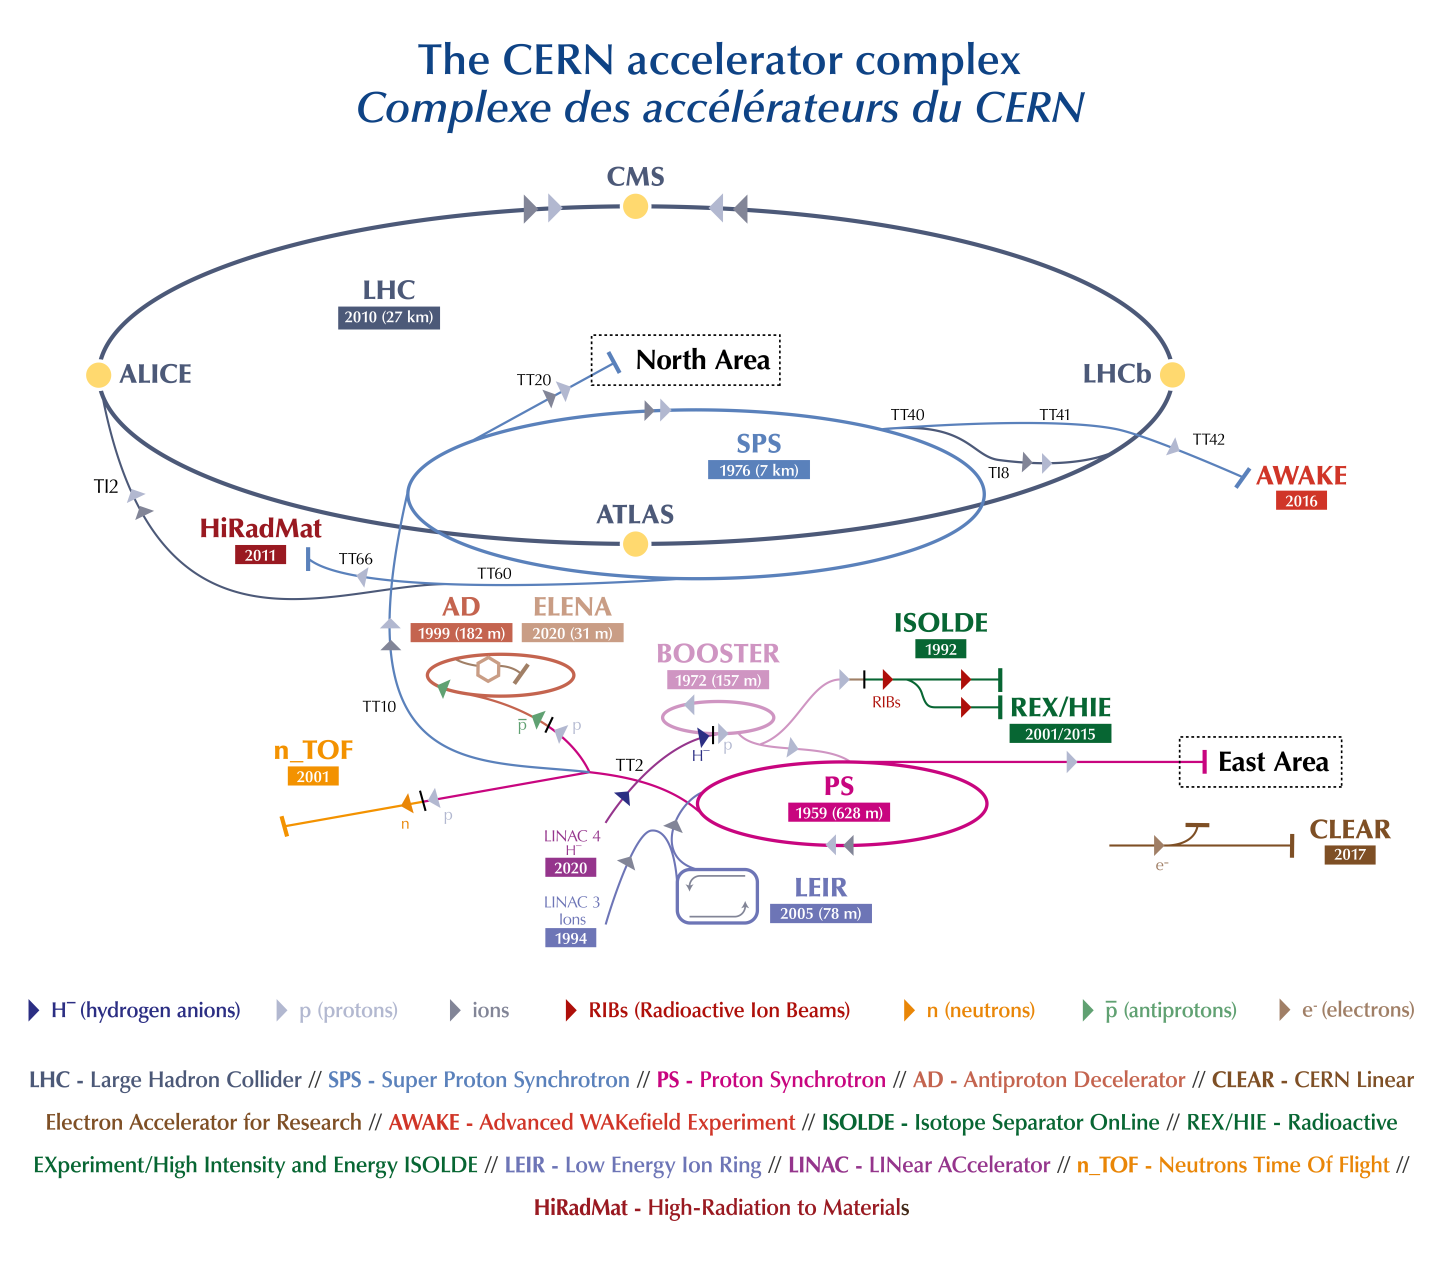
\includegraphics[width=0.75\textwidth]{cern_complex}
	\caption{The CERN accelerator complex. © 2019-2020 CERN.}
	\label{fig:cern_accelerator_complex}
\end{figure}

Most of the physical processes of interest to high energy physics (HEP) are extremely rare.
This necessitates that the overarching goal of collider experiments be to maximize the amount of collisions observed.
At the LHC this is achieved via an elaborate scheme called Batch Compression Merging and Splitting (BCMS) that determines when and how the proton bunches are split and the beam is compressed at each stage of the proton accelerator chain described above.

\subsection{Luminosity}
\newcommand{\CollRate}{\ensuremath{R_{\mathrm{inelastic}}}}
\newcommand{\InstLumi}{\ensuremath{\mathcal{L}_{\mathrm{inst}}}}
\newcommand{\InelXsec}{\ensuremath{\sigma_{\mathrm{inelastic}}}}

The scientific potential of a particle collider experiment can be quantified by its center-of-mass energy and the number of inelastic collisions it produces per unit time
\begin{equation}
\CollRate = \InstLumi\ \InelXsec,
\label{eqn:collision_rate}
\end{equation}
where \InstLumi\ is the \textit{instantaneous luminosity} and \InelXsec\ is the \textit{inelastic scattering cross section} of the particle collisions. The units of \InstLumi\ are events per time per area, and the units of \InelXsec\ are area per event. In classical terms \InelXsec\ represents the area transverse to the relative motion of the two scattering particles within which they must meet in order to scatter from each other. From the perspective of QFT, \InelXsec\ is more accurately described as the scattering event probability. Given these definitions, \InstLumi\ quantifies the part of the collision rate that is determined by the collider itself.
The peak instantaneous luminosity delivered to the ATLAS detector during Run-2 of the LHC was $21.0 \times 10^{33}\ \mathrm{cm}^{-2}\ \mathrm{s}^{-1}$.

In terms of the properties of storage rings like the LHC the rate can also be written as
\begin{equation}
\CollRate = n_b f_{\mathrm{rev}} \langle \mu \rangle
\label{eqn:collision_rate_beam}
\end{equation}
where $f_{\mathrm{rev}}$ is the revolution frequency of the ring\footnote{At the LHC the protons traverse the ring at a revolution frequency of 11245.5 Hz.}, $n_b$ is the number of colliding bunches and $\langle \mu \rangle$ is the average number of simultaneous inelastic interactions per bunch crossing.
Thus the instantaneous luminosity can be re-written as
\begin{equation}
\InstLumi = \frac{n_b f_{\mathrm{rev}} \langle \mu \rangle}{\InelXsec}.
\label{eqn:inst_lumi_ring}
\end{equation}

An alternative way to express \InstLumi\ in terms of beam quantities allows the luminosity to be measured\cite{Grafstrom:2015foa}. In the case of symmetric, Gaussian beams the instantaneous luminosity can be expressed as
\begin{equation}
\InstLumi = \frac{n_b f_{\mathrm{rev}} N_1 N_2}{4\pi \Sigma_x \Sigma_y},
\label{eqn:inst_lumi_beam}
\end{equation}
where $\Sigma_x, \Sigma_y$ are the convolved beam size $\left(\Sigma_{x/y} = \sqrt{\sigma_{x/y,1}^2 + \sigma_{x/y,2}^2}\right)$ in the $x$/$y$ plane and $N_1$/$N_2$ are the number of protons in each bunch.
The values for $\Sigma_{x/y}$ are measured with the ATLAS detector during special data-taking periods \cite{ATLAS-CONF-2019-021} using techniques known as van der Meer scans, during which a small separation is induced and varied along the axes transverse to the collisions. In addition to the quantities shown in Eq.~\ref{eqn:inst_lumi_beam} and Eq.~\ref{eqn:inst_lumi_ring}, the optimization of $\InstLumi$ at the LHC includes consideration of beam properties such as the crossing angle $(\theta_c)$ and longitudinal compression $(\beta^*)$ around the interaction point (IP).

Ultimately the \textit{integrated luminosity} $L$ determines the number of events observed by a collider experiment.
\begin{equation}
L = \int \InstLumi(t)\ dt
\label{eqn:integrated_lumi}
\end{equation}
where the integral is over the total stable data-taking uptime of the detector.
For a given rare physics process $x$ the expected number of observed events for a given integrated luminosity $L$ is
\begin{equation}
N_{\mathrm{events}}^{x} = \epsilon_x \sigma_x L
\label{eqn:nobs_events}
\end{equation}
where $\sigma_x$ is the cross section (fixed by Nature), $\epsilon_x$ is the detection efficiency which is a product of both the geometrical coverage of the detector and analysis selection efficiency.
Optimization of $\epsilon_x$ for both SM measurements and BSM searches is one of the primary focal points for most HEP researchers, but the primary limitation will always be the integrated luminosity delivered by the particle collider.

\subsection{Operational History}
The LHC experimental program follows a detailed timeline of data taking periods known as ``Runs'' interspersed with longer shutdown periods used to repair and upgrade the experiments and the accelerator.
At the LHC these data-taking periods typically take place between April and November during non-shutdown years.
Since Run 1 began in 2011 the LHC has followed a gradual trend of increasing center-of-mass energy $(\sqrt{s})$ and instantaneous luminosity.
The nominal design luminosity has already been surpassed by a factor of two, and the nominal design value of $\sqrt{s} = 14$\ TeV will be achieved for Run 3 and beyond.
In 2016 the CERN Council approved a roadmap (see Fig.~\ref{fig:lhc_timeline}) for twenty more years of LHC physics which will ultimately surpass the nominal design luminosity by up to a factor of seven.
At the time of the writing of this thesis the LHC is in the midst of the second long shutdown (LS2).

\begin{figure}
	\centering
	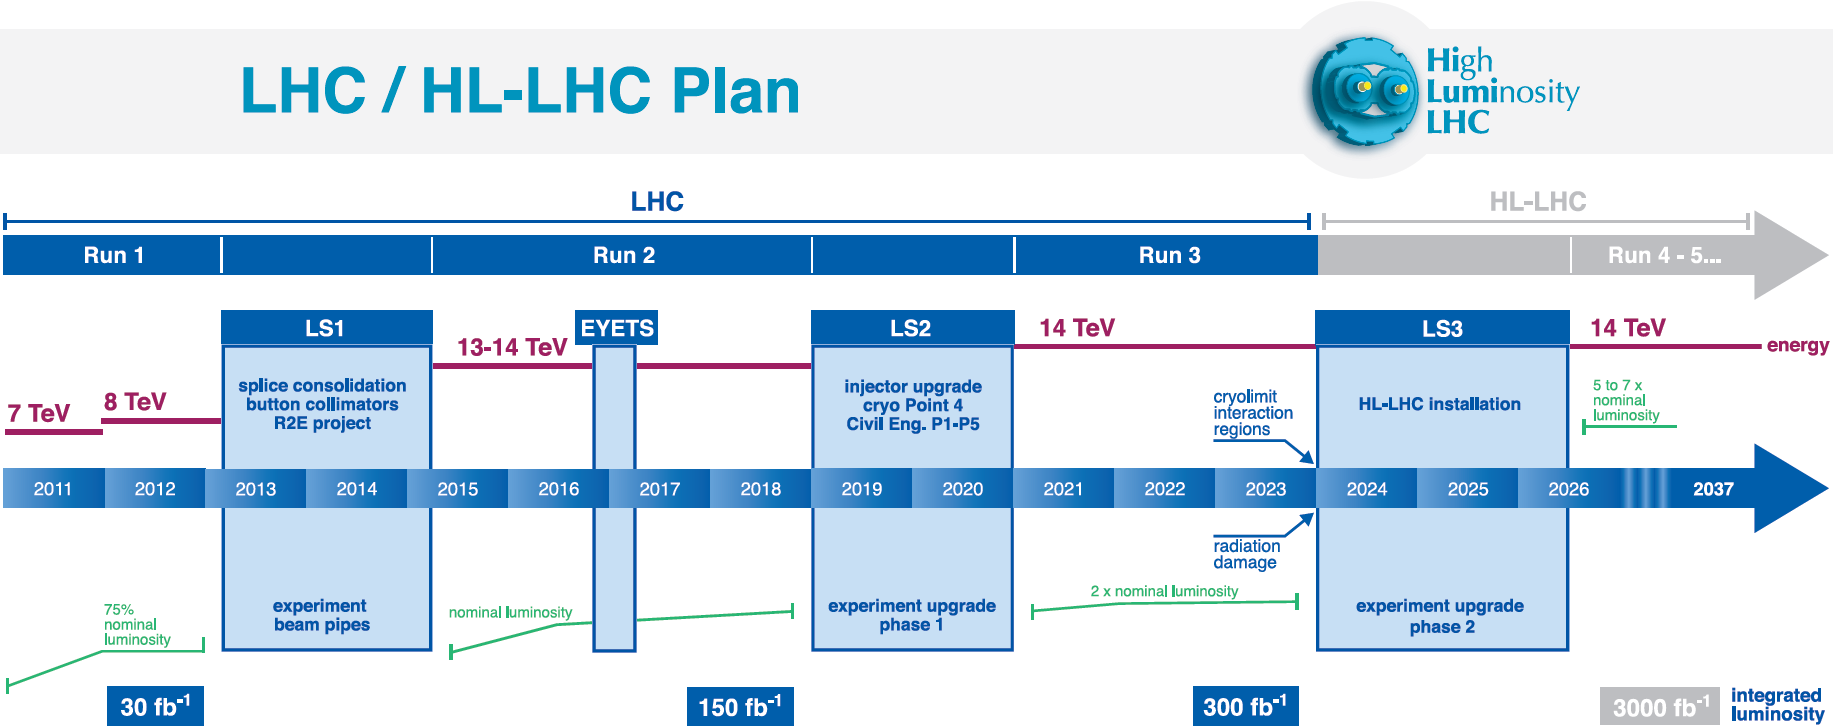
\includegraphics[width=0.9\textwidth]{lhc_timeline}
	\caption{Timeline of the LHC program up to the high-luminosity LHC (HL-LHC). © CERN}
	\label{fig:lhc_timeline}
\end{figure}

The cumulative luminosity delivered to the ATLAS detector so far as a function of time for each separate year can be seen in Fig.~\ref{fig:int_lumi_vs_year}.
The final measured integrated luminosity luminosity values for Run-2, along with their uncertainties, are shown in Table~\ref{tab:lumi_vs_period}.

\znote{show history of runs/shutdowns}
% \eqref{eqn:equation}

\begin{figure}
	\centering
	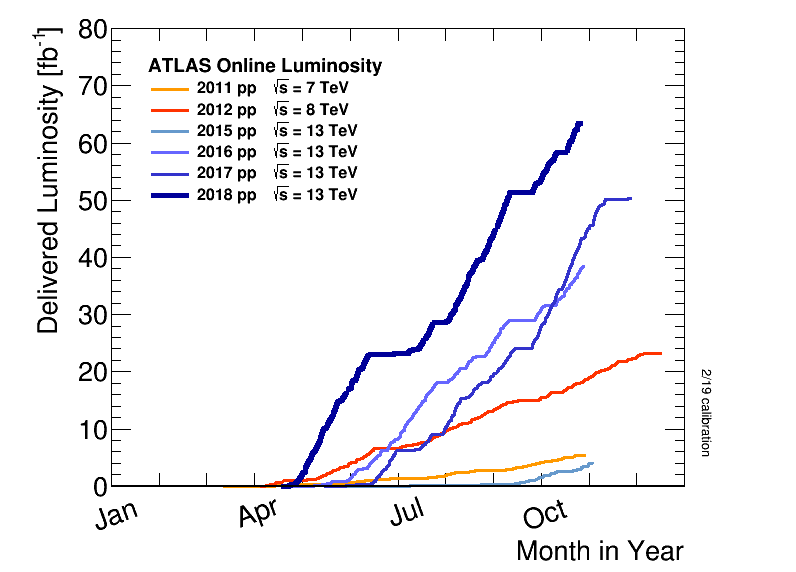
\includegraphics[width=0.65\textwidth]{int_lumi_vs_year}
	\caption{Cumulative luminosity versus day delivered to ATLAS during stable beams for high energy p-p collisions. © CERN}
	\label{fig:int_lumi_vs_year}
\end{figure}

\begin{table}
\centering
\begin{tabular}{|c|c|} 
\hline
Period & Luminosity [fb$^{-1}$] \\
\hline\hline
2015+16 & 36.2 $\pm$ 0.8 \\ 
\hline
2017 & 44.3 $\pm$ 1.0 \\
\hline
2018 & 58.5 $\pm$ 1.2 \\
\hline\hline
Run-2 & 139.0 $\pm$ 2.4 \\
\hline
\end{tabular}
\caption{
    The total luminosity delivered by the LHC to the ATLAS detector during Run-2.
    Values are taken from the ATLAS online luminosity determination measurements described in Ref.~\cite{ATLAS-CONF-2019-021}.
}
\label{tab:lumi_vs_period}
\end{table}

\section{ATLAS Detector}

\subsection{Overview}
The ATLAS detector is the largest volume detector ever constructed for a particle collider.
It is cylindrically shaped with a diameter of 25 m, a length of 46 m, and located 100 m underground at the first IP of the LHC.
The total weight of the detector is 7,000 metric tonnes, which is equivalent to almost ten thousand Volkswagen Beetles.
The major ATLAS detector components can be seen in Fig.~\ref{fig:atlas_detector_overview}.

The ATLAS detector is composed of several subdetectors which measure different properties of the particles which emerge from the proton-proton collisions around the IP.
The subdetectors closest to the beam line are the inner tracking detectors (Sec.~\ref{sec:inner_detector}) which measure with high precision the flight paths of charged particles.
Continuing outwards, the next subdetectors are the calorimeters (Sec.~\ref{sec:calorimeters}), of which there are two types: electromagnetic and hadronic.
These calorimeters measure the energy deposited by both charged and neutral particles as they are slowed or, most often, completely stopped by the calorimeter detector material.
The muon spectrometer (Sec.~\ref{sec:muon_spectrometer}) is the outermost subdetector and provides additional measurements along trajectory of muons.

\begin{figure}
	\centering
	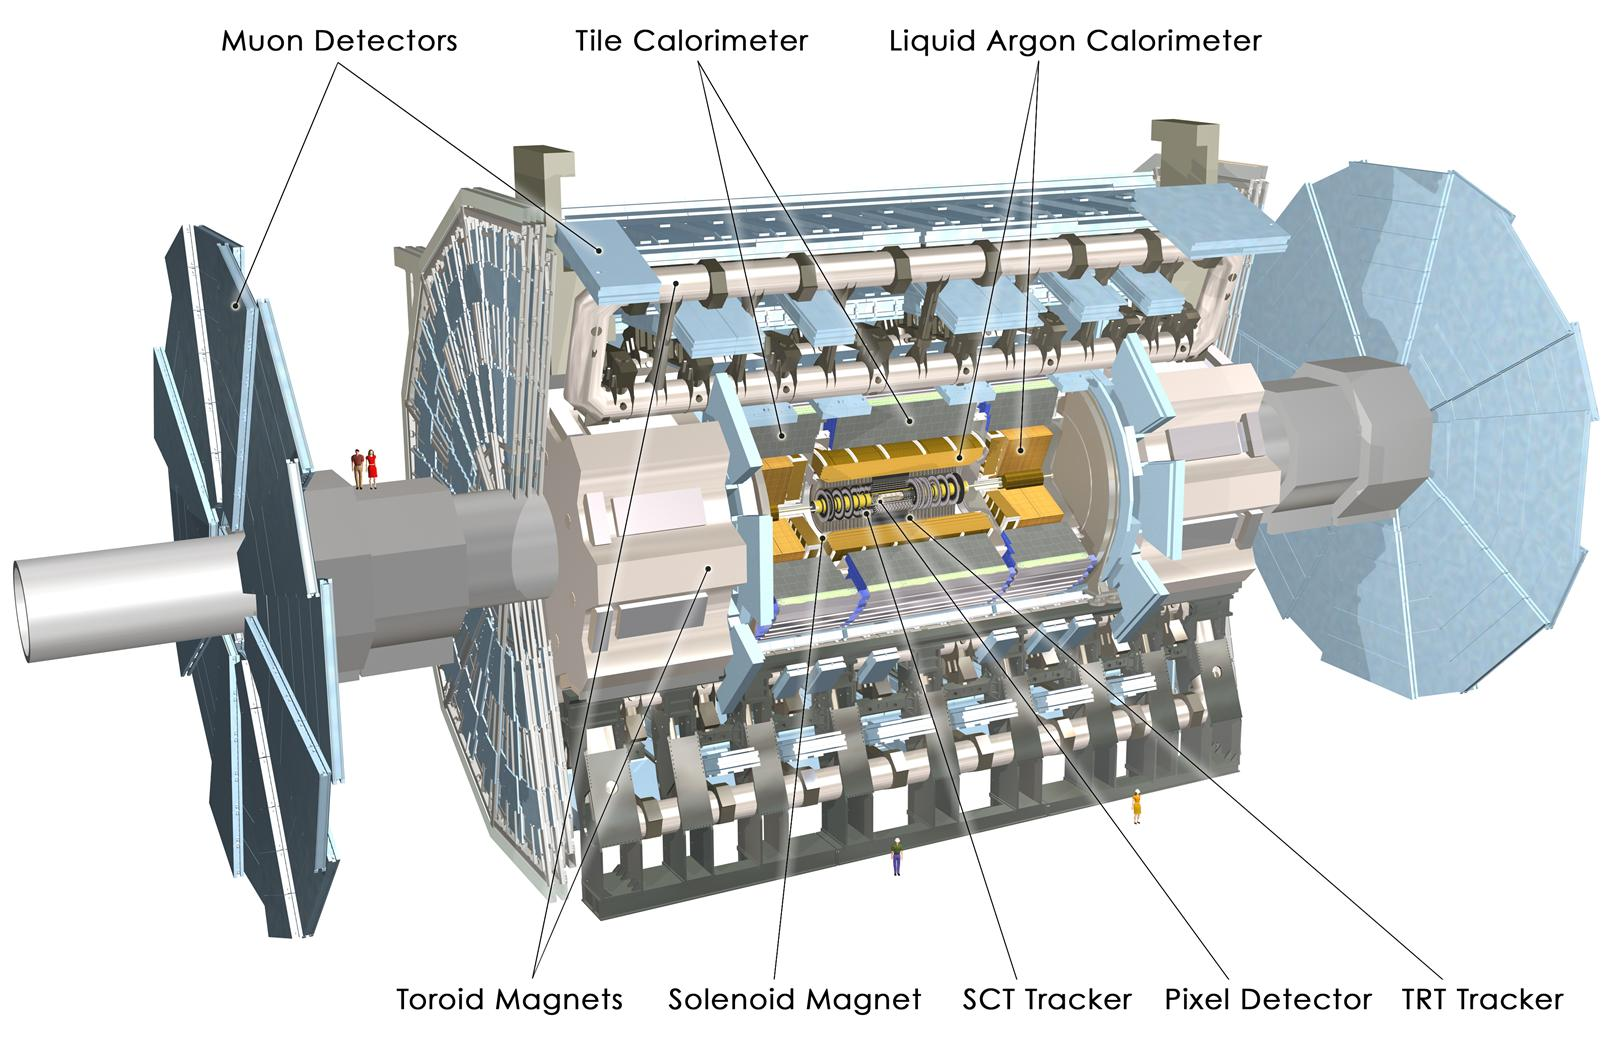
\includegraphics[width=0.8\textwidth]{entire_detector}
	\caption{
	A computer-generated cutout view of the ATLAS detector illustrating all of the various subdetector components.
	Note the human beings included for scale on the left.
	© 2008 CERN.
	}
	\label{fig:atlas_detector_overview}
\end{figure}

\subsection{Coordinate System}
The ATLAS detector uses a right-handed coordinate system as illustrated in Fig.~\ref{fig:atlas_coordinate_system}.
The $x$-axis points towards the center of the LHC ring, the $y$ axis points upwards away from the center of the earth and the $z$-axis points along the beam line.
When describing the products of a collision event it is often more useful to use a set of polar coordinates defined relative to  this Cartesian coordinate system.

\begin{figure}
	\centering
	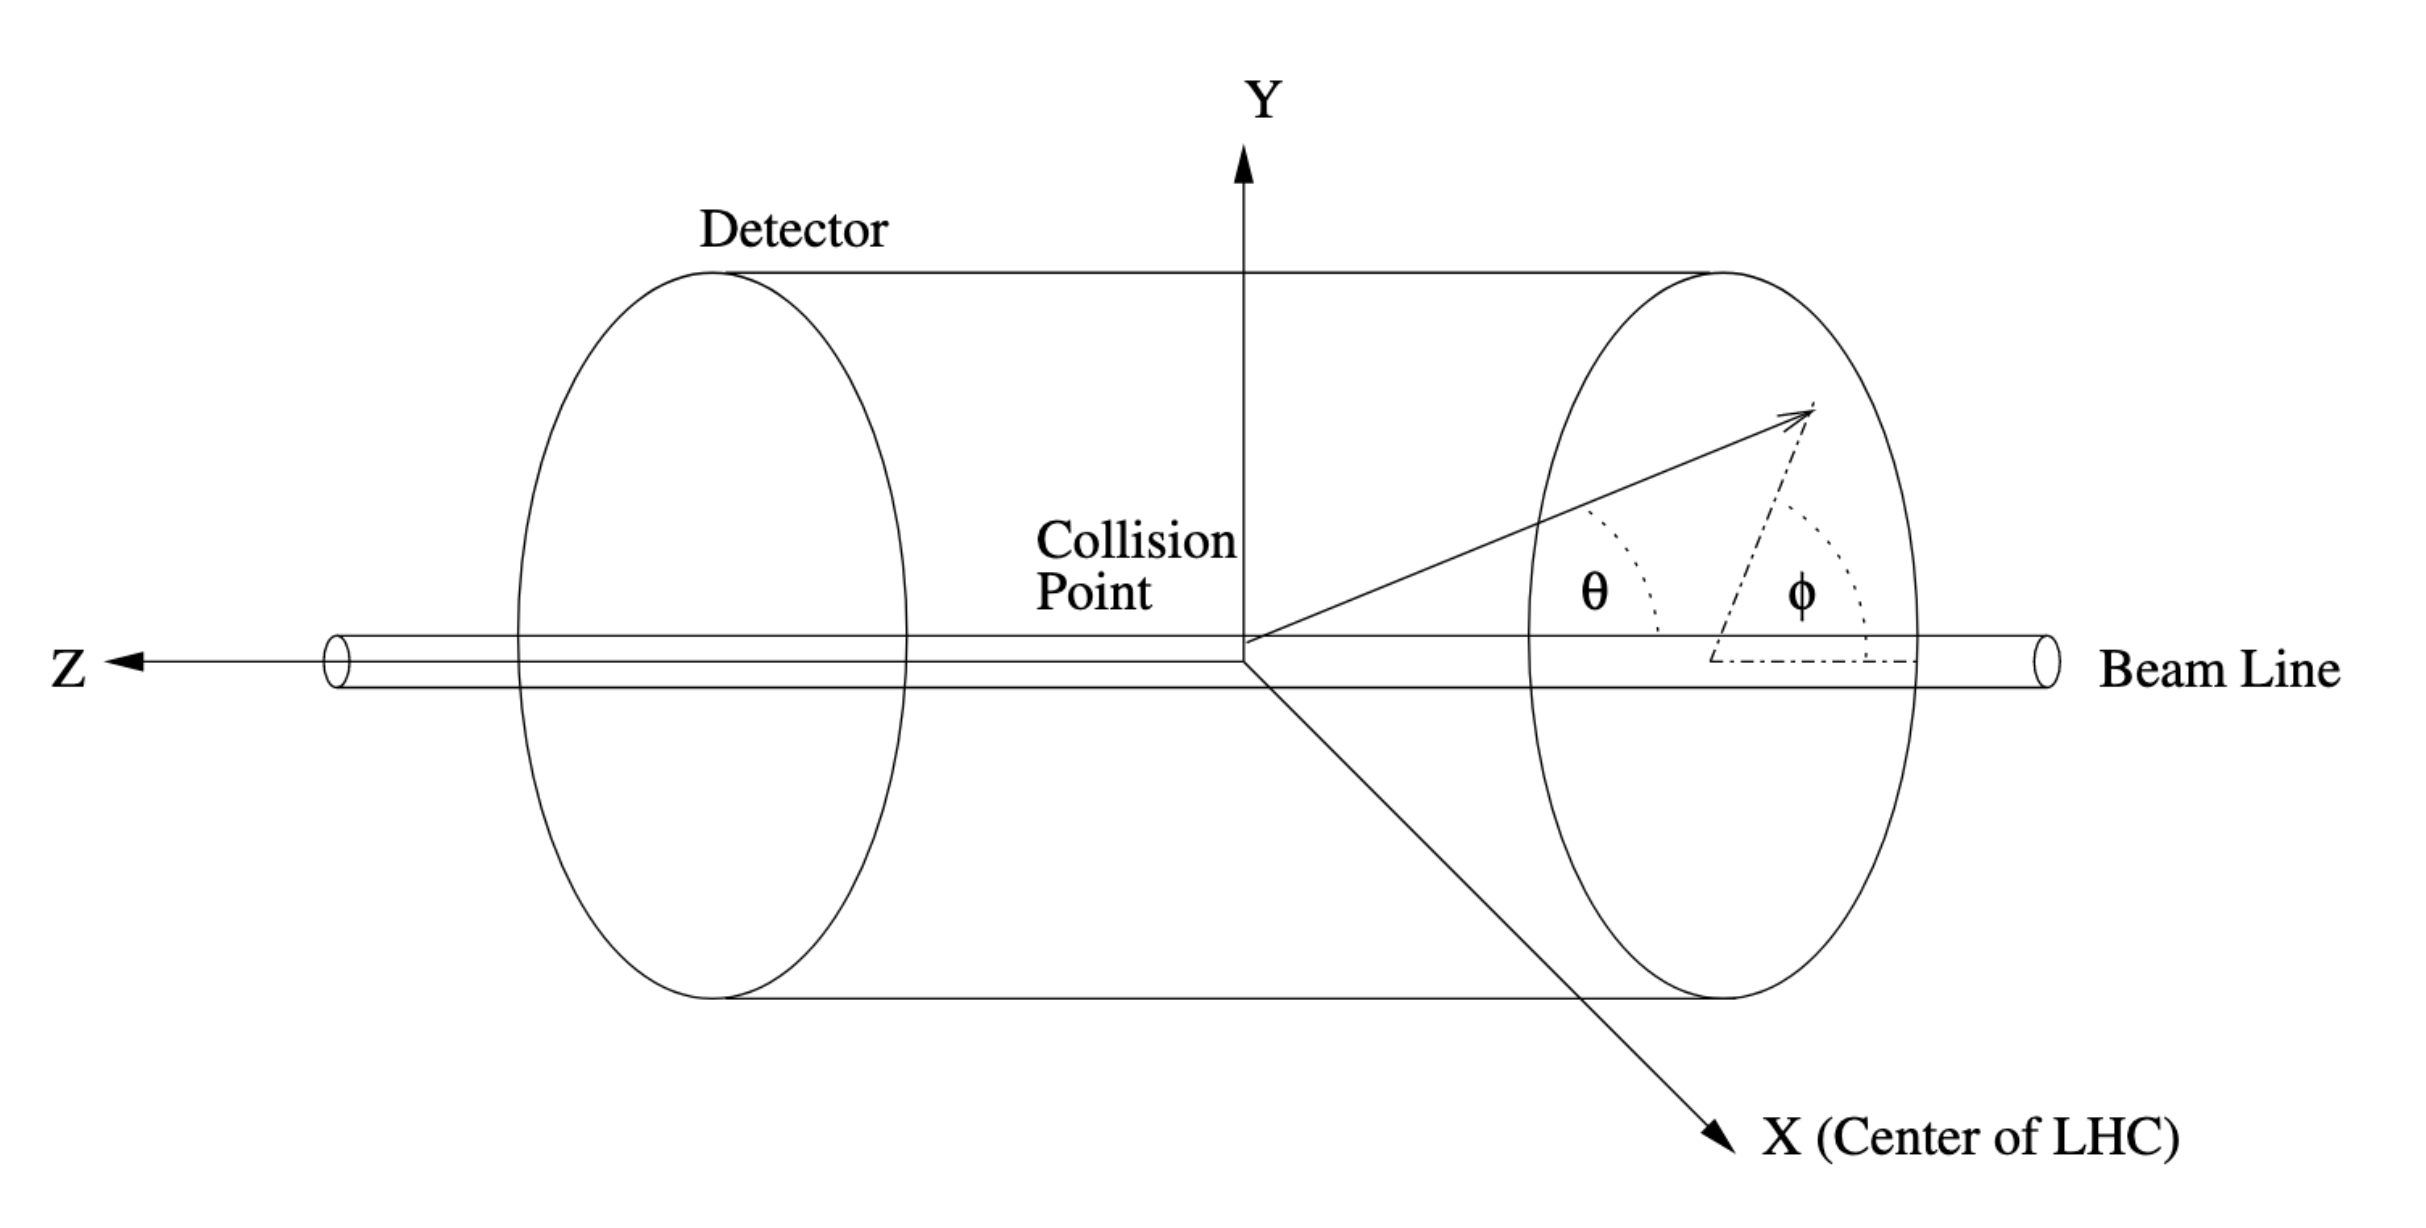
\includegraphics[width=0.8\textwidth]{atlas_coordinate_system}
	\caption{ Illustration of the ATLAS coordinate system \cite{Schott_2014}. }
	\label{fig:atlas_coordinate_system}
\end{figure}

These polar coordinates are defined as follows:
\begin{align}
\phi &= \arctan\left( {\frac{y}{x}} \right) \\
\theta &= \arctan \left( {\frac{z}{\sqrt{x^2+y^2}}} \right)
\label{eqn:polar_coordinates}
\end{align}
where $\theta$ is the \textit{polar} angle and $\phi$ is the \textit{azimuthal} angle.
The polar angle $\theta$ is not convenient for use in particle physics because it is not invariant under boosts along the beam line axis. For this reason a related quantity called the \textit{rapidity} $(y)$ is defined as
\begin{equation}
y = \frac{1}{2} \ln \left( \frac{E + p_z}{E-p_z} \right)
\label{eqn:rapidity}
\end{equation}
and is invariant under boosts along the z-axis. However, due to the dependence of $y$ on energy/momentum, a purely geometric quantity called \textit{pseudorapidity} is most often used in its place, defined by
\begin{equation}
\eta = -\ln \left(\tan\left( \frac{\theta}{2} \right) \right)
\label{eqn:pseudorapidity}
\end{equation}
which is equivalent to rapidity in the case of massless or highly energetic particles.
A visualization of the distribution of $\eta$ values is illustrated in Fig.~\ref{fig:pseudorapidity}.
A measure of distance\footnote{The radial distance from the beam center $\left(R = \sqrt{x^2 + y^2}\right)$ is also commonly used in discussing tracking and the Inner Detector.} between particles in the $\eta-\phi$ ``plane'' is commonly used and defined as
\begin{equation}
\Delta R = \sqrt{(\Delta \eta)^2 + (\Delta \phi)^2}
\label{eqn:deltaR}
\end{equation}

\begin{figure}
	\centering
	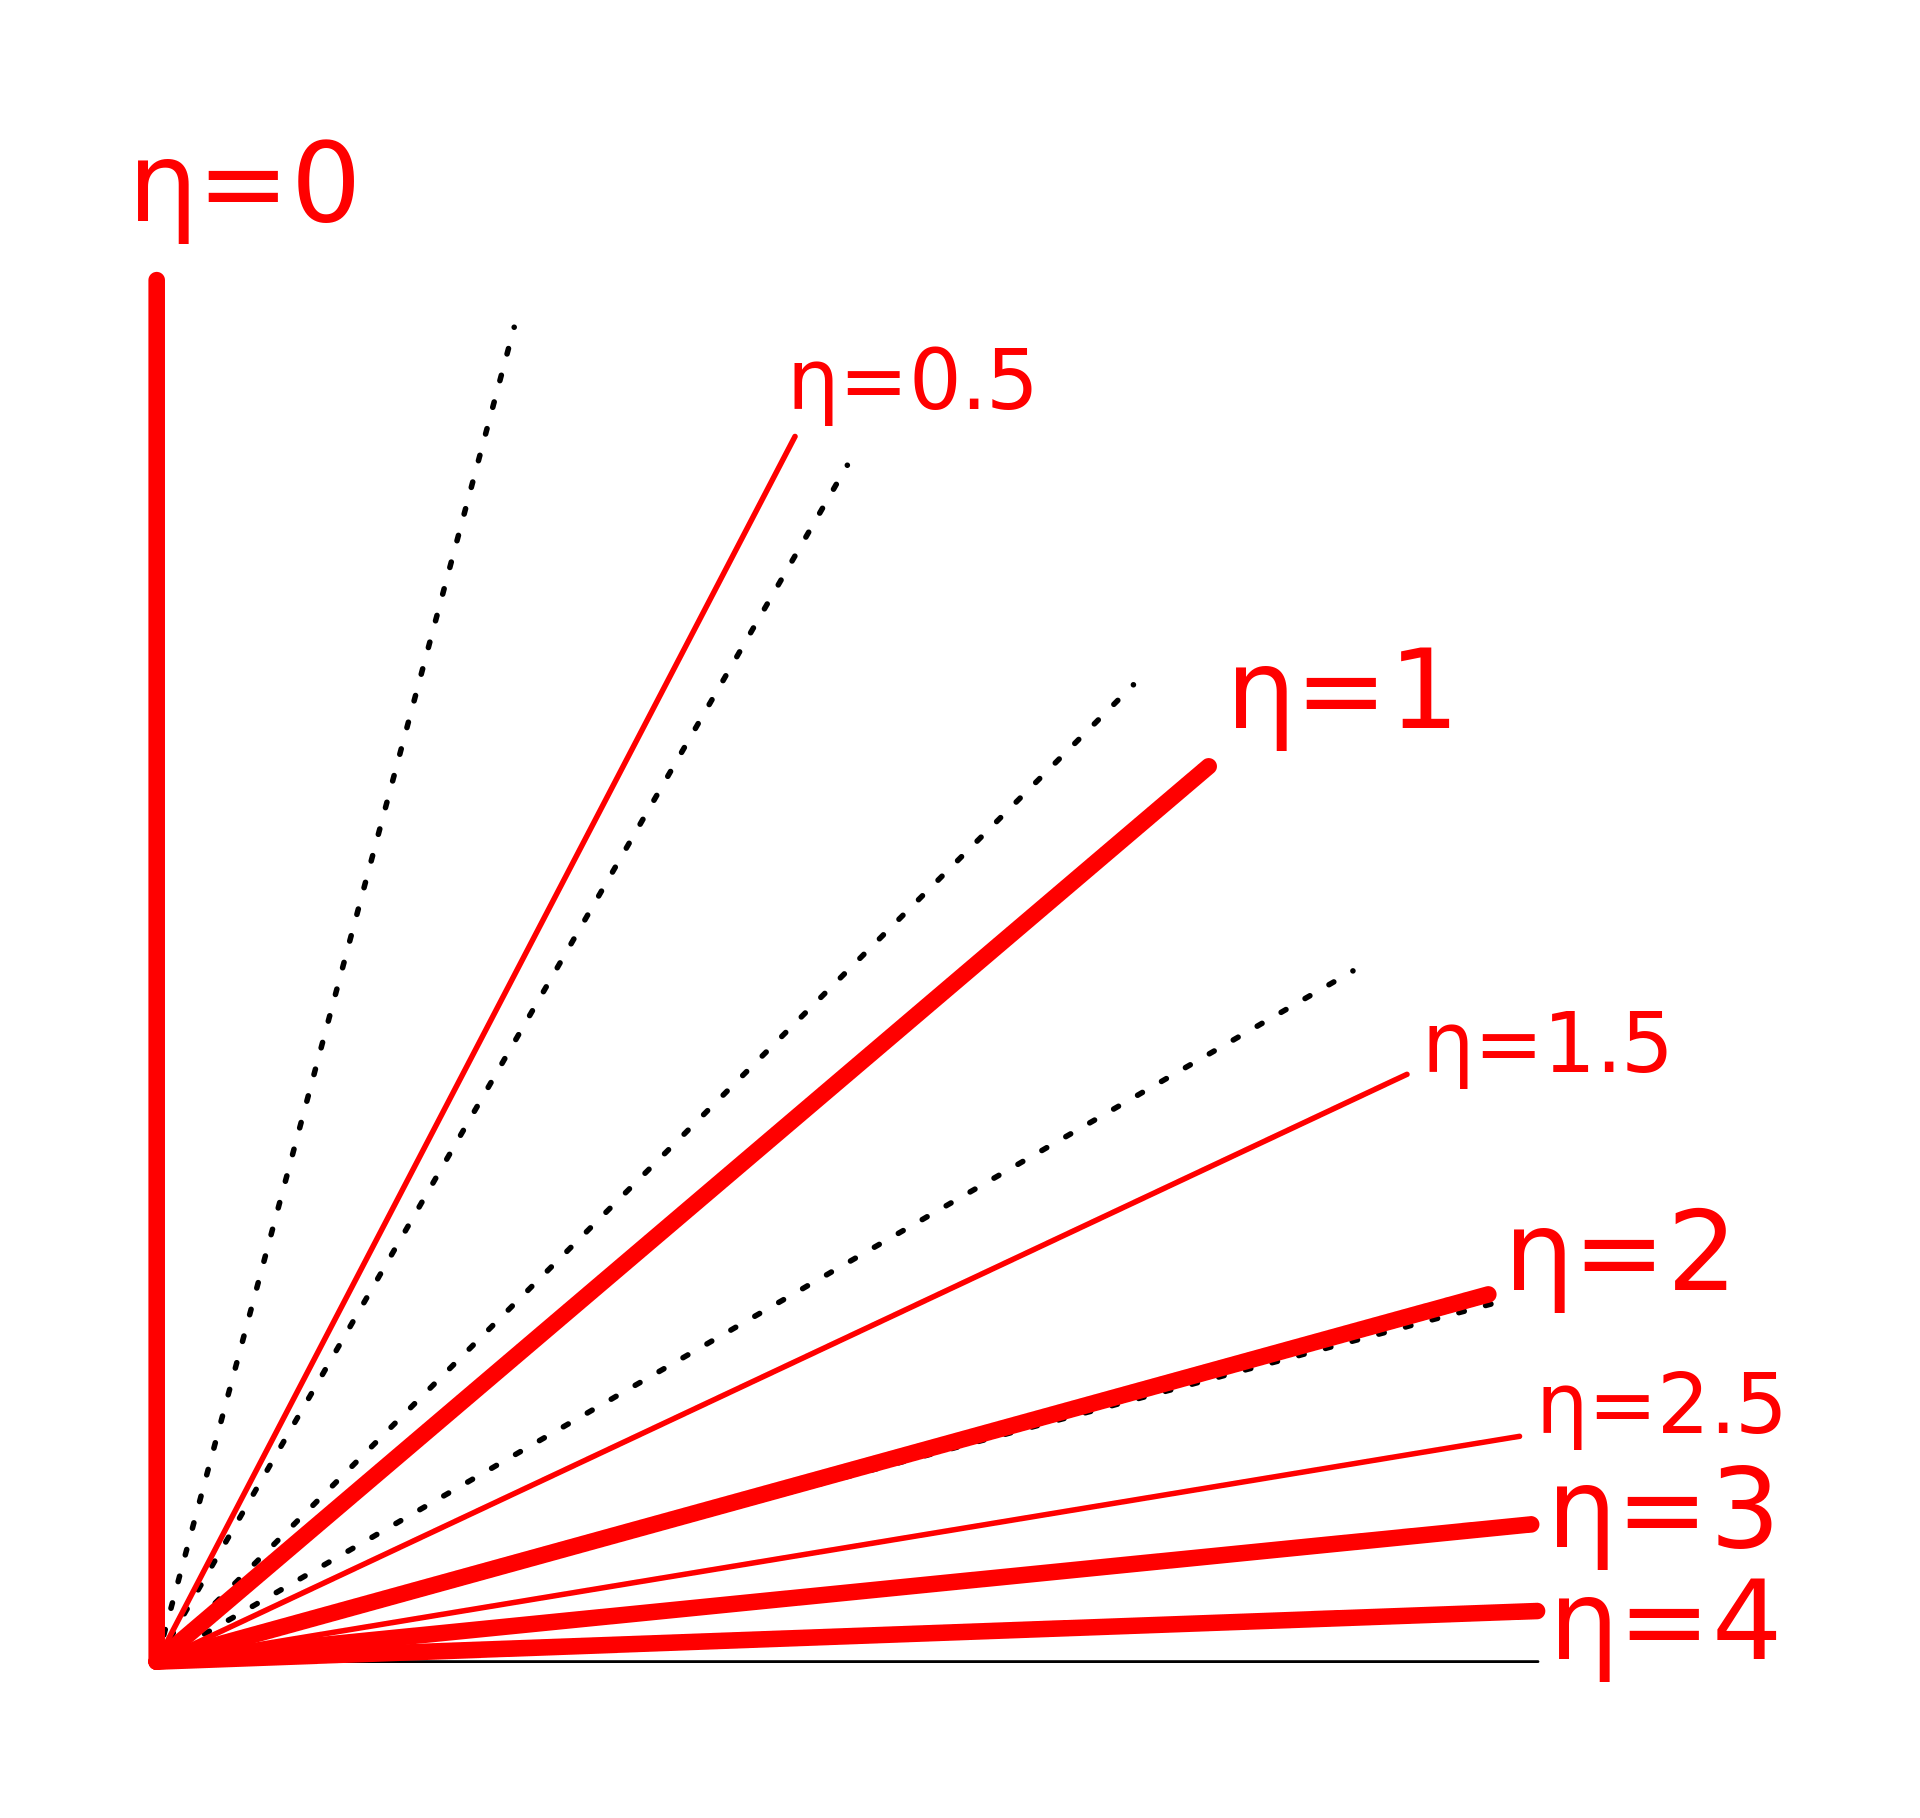
\includegraphics[width=0.4\textwidth]{pseudorapidity}
	\caption{Example values of pseudorapidity. The value of $\eta$ approaches infinity as the beam line ($z$-axis, towards the right) is approached. A value of $\eta = 0.5$ corresponds to a polar angle of 27.5 degrees, $\eta = 1.0$ corresponds to 49.6 degrees, $\eta = 1.5$ corresponds to 64 degrees, $\eta = 4$ corresponds to 87.9 degrees. }
	\label{fig:pseudorapidity}
\end{figure}

When measuring the properties of collision products, the momentum they possess along the beam line is less important than their momentum perpendicular to the beam line. This is because the momentum of the colliding particles along the beam line is unknown, while the perpendicular momentum is purely a consequence of whatever physics occurred during the collision due to conservation of momentum.
For this reason the \textit{transverse momentum} and \textit{transverse energy} are more often used instead, and defined as
\begin{align}
p_T &= \sqrt{p_x^2 + p_y^2} \\
E_T &= E \sin(\theta) = E \sinh(\eta).
\label{eqn:transverse_momentum_energy}
\end{align}
Both of these quantities are invariant with respect to boosts along the beam axis.

\subsection{Inner Detector}
\label{sec:inner_detector}
The ATLAS Inner Detector (ID) \cite{CERN-LHCC-97-016} \cite{ATLAS-TDR-2008} is a tracking detector that records the paths taken by charged particles as they emerge from the collisions around the IP.
Two of the primary design goals for the ID are to provide a transverse momentum resolution of $\frac{\sigma_{p_T}}{p_T} = 0.05\% \times p_T \oplus 1\%$ and a transverse impact parameter resolution of $10 \mu$m for high momentum partices in the central pseudorapidity region \cite{ATLAS-TDR-2008}.

The ID is itself composed of four separate concentric detectors: The Insertable B-Layer (IBL), the Pixel detector, the Semiconductor Tracker (SCT), and the Transition Radiation Tracker (TRT).
These individual subdetectors can be seen in Fig.~\ref{fig:inner_detector_cgi}.
A more detailed view of the sensor components from each subdetector within the Inner Detector is shown in Fig.~\ref{fig:inner_detector_zoomed_cgi}.
The active area of the Inner Detector extends up to $|\eta| < 3$ for the IBL, $|\eta| < 2.5$ for the Pixel/SCT, and $|\eta| < 2.0$ for the TRT.

The entire Inner Detector is immersed in an axial symmetric $2T$ magnetic field provided by an enclosing solenoid magnet.
The magnet is 5.3 m long, 2.4 m in diameter, 4.5 cm thick and weighs approximately 5 metric tonnes.
The purpose of the magnetic field is to bend the trajectories of charged particles\footnote{This bending is achieved via the Lorentz Force, which bends charged particle motion in the plane perpendicular to that of a magnetic field.} in the $x-y$ plane as they move through the detector so that momentum and charge can be deduced from the resulting path curvature.
The path of charged particles with low momentum $(< 400 \mathrm{MeV})$ are so tightly curved by the magnetic field that they never move far enough from the IP in the radial direction to interact with even the first detector layer.

\begin{figure}
	\centering
	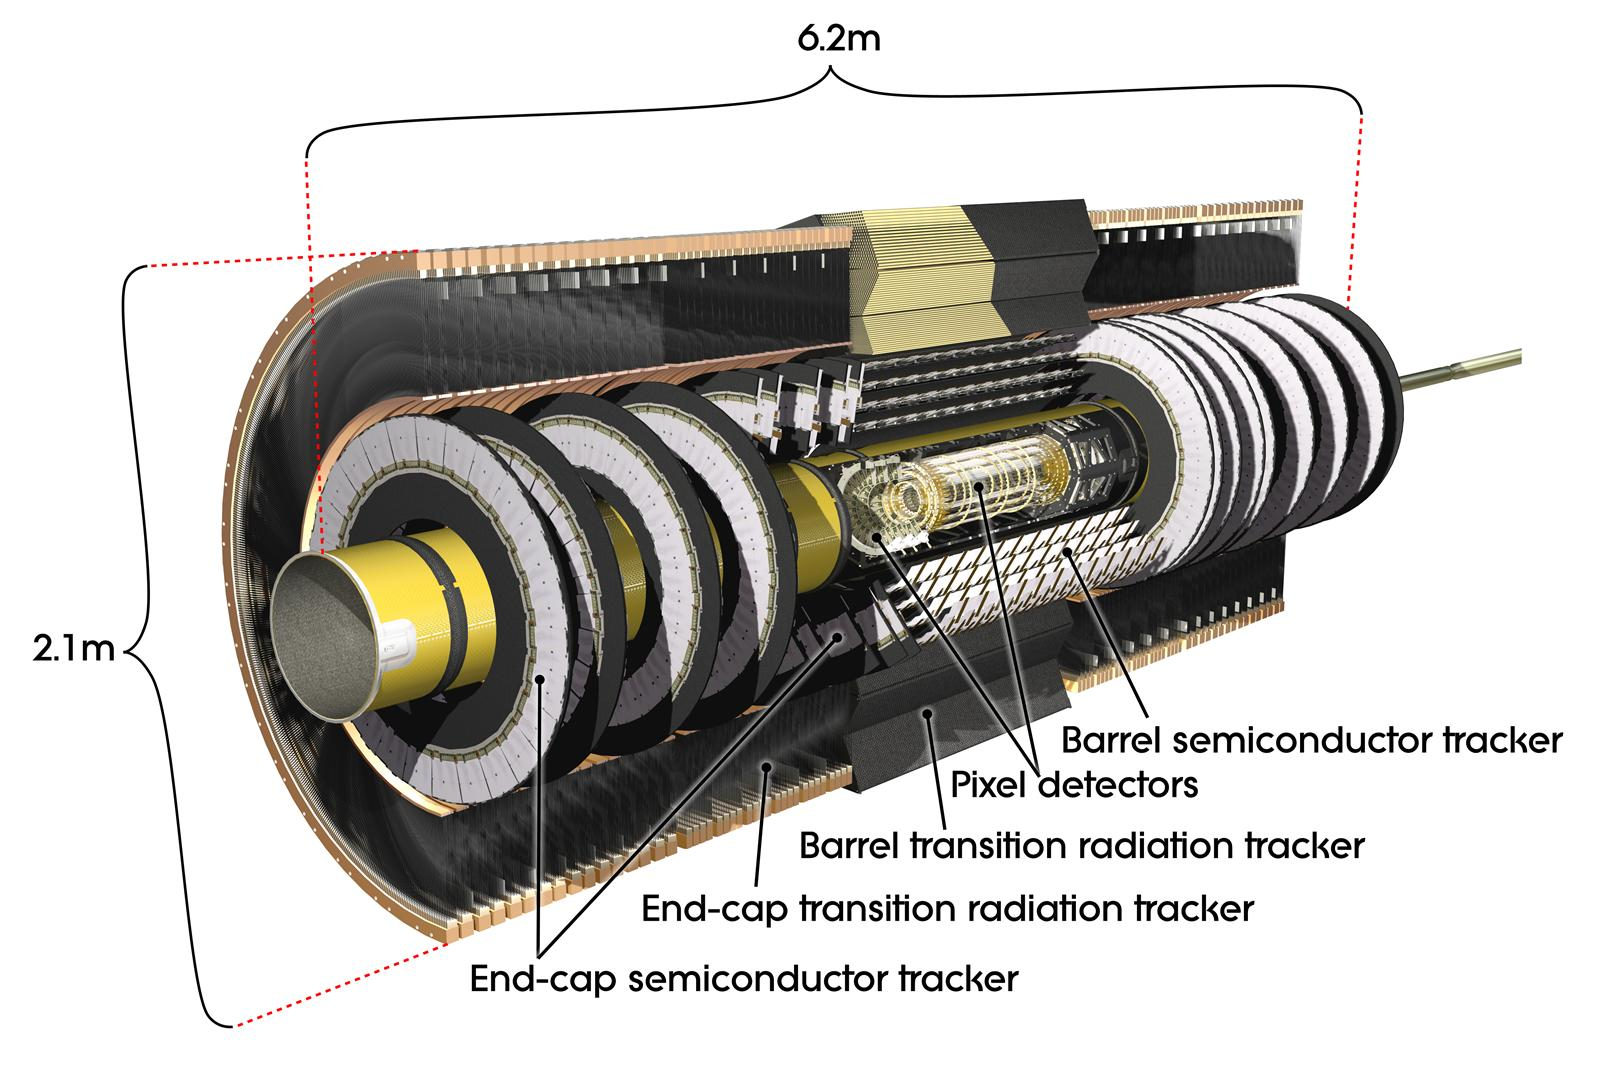
\includegraphics[width=0.75\textwidth]{inner_detector}
	\caption{A computer generated cutaway image displaying the components of the ATLAS Inner Detector. © 2014 CERN.}
	\label{fig:inner_detector_cgi}
\end{figure}

The IBL, Pixel and SCT detectors all operate via the same underlying detection technology: excitation of p-n junctions in silicon.
When a charged particle passes through a portion of the silicon and deposits energy via collision, silicon is ionized and electron-hole pairs are created.
These electrons then drift and create a current due a bias voltage that is applied across the silicon.
The magnitude of the current produced depends on the energy of the incident particle, as more electron-hole pairs are produced for a higher momentum particle.

The reconstruction of the particle trajectory is of utmost importance because the curvature of the particle path allows for the determination of both the charge and momentum of the particle.
One of the primary reasons the Inner Detector is situated as the closest subdetector to the beamline is so that it may reconstruct the trajectory of even short-lived particles that decay before reaching the outer layers of the detector.
This improves the quality of primary vertex reconstruction and makes it possible to reconstruct secondary vertices. 
%TODO cite vertex reco section for explanation of vertex lingo

\begin{figure}
	\centering
	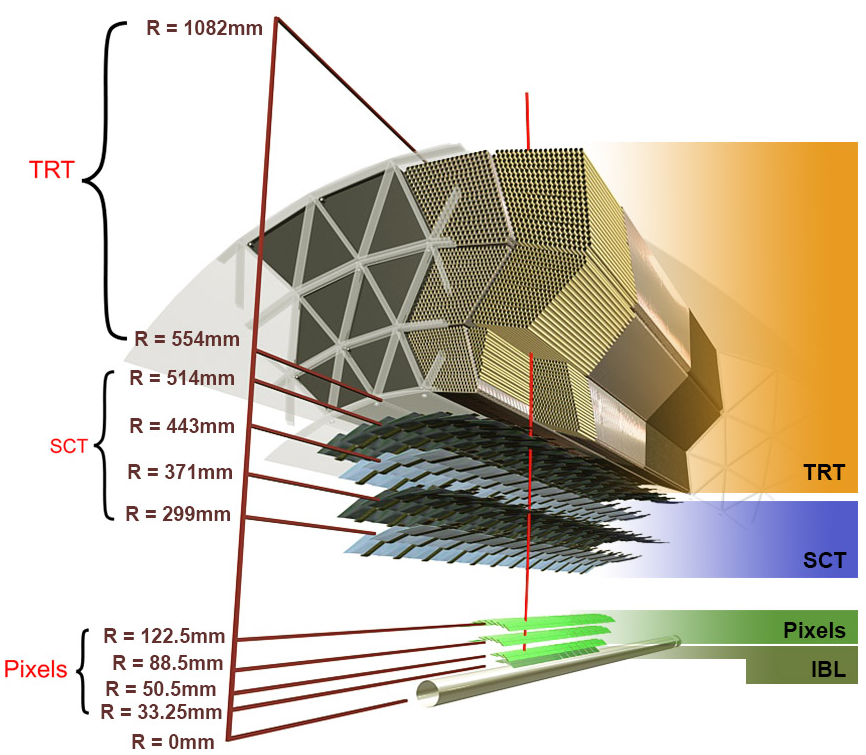
\includegraphics[width=0.6\textwidth]{inner_detector_zoomed}
	\caption{Exploded view of the sensor components of the IBL, Pixel, SCT, and TRT layers of the ATLAS Inner Detector. © 2014 CERN.}
	\label{fig:inner_detector_zoomed_cgi}
\end{figure}

\subsubsection{Insertable B-Layer (IBL)}
The IBL~\cite{Capeans:1291633, Abbott:2018ikt} is the innermost and newest layer of the Inner Detector, installed in 2014 during the first long shutdown period of the LHC.
The purpose of the IBL is primarily to improve the measurement resolution of the transverse and longitudinal impact parameters of tracks, particularly in the face of increased pileup and luminosity during the HL-LHC phase.
These impact parameters are of crucial importance for vertex reconstruction and the identification of $b$-jets. \znote{cite relevant sections}

The IBL is located at an average radial distance of 33 mm from the center of the beam pipe, covers $332$mm in the z-direction, and extends the active tracking area up to $|\eta| < 3$ compared to the $|\eta| < 2.5$ coverage of the ID without the IBL.
The planar pixel sensors in the central $|\eta|$ region of the IBL have an instrinsic resolution of approximately $0.01$ to $0.04$mm in $R-\phi$ and $0.6$ to $1.8$mm in $z$, which allows for precise measurements of charged particle momentum.

\subsubsection{Pixel}
The Pixel detector barrel is composed of three concentric cylindrical layers of silicon semiconductor staves at radial distances of 50.5, 88.5 and 122.5 mm which extend to $|z| \approx 400$ mm on either side.
Two end-cap sections consisting of three semiconductor disks are situated at each end perpendicular to the beam axis at $|z| = 495, 580, 650$ mm.
The Pixel detector contains over 80 million sensors in total, each with an intrinsic resolution of approximately $8\mu$m in $R-\phi$ and $75\mu$m in $z$.
These pixel sensors are divided into 1744 modules of 46080 pixels each with an area of $\approx$ 10cm, covering a total area of 1.7 $\mathrm{m}^2$.
The barrel layers cover $|\eta| < 2$ and contain 1456 modules, while the end caps extend coverage to $|\eta| < 2.5$ and contain 288 modules.
The barrel layers are arranged in a turbine-like fashion with an overlap in $\phi$, as shown in Fig.~\ref{fig:pixel_ibl_cross_section}.

\begin{figure}
	\centering
	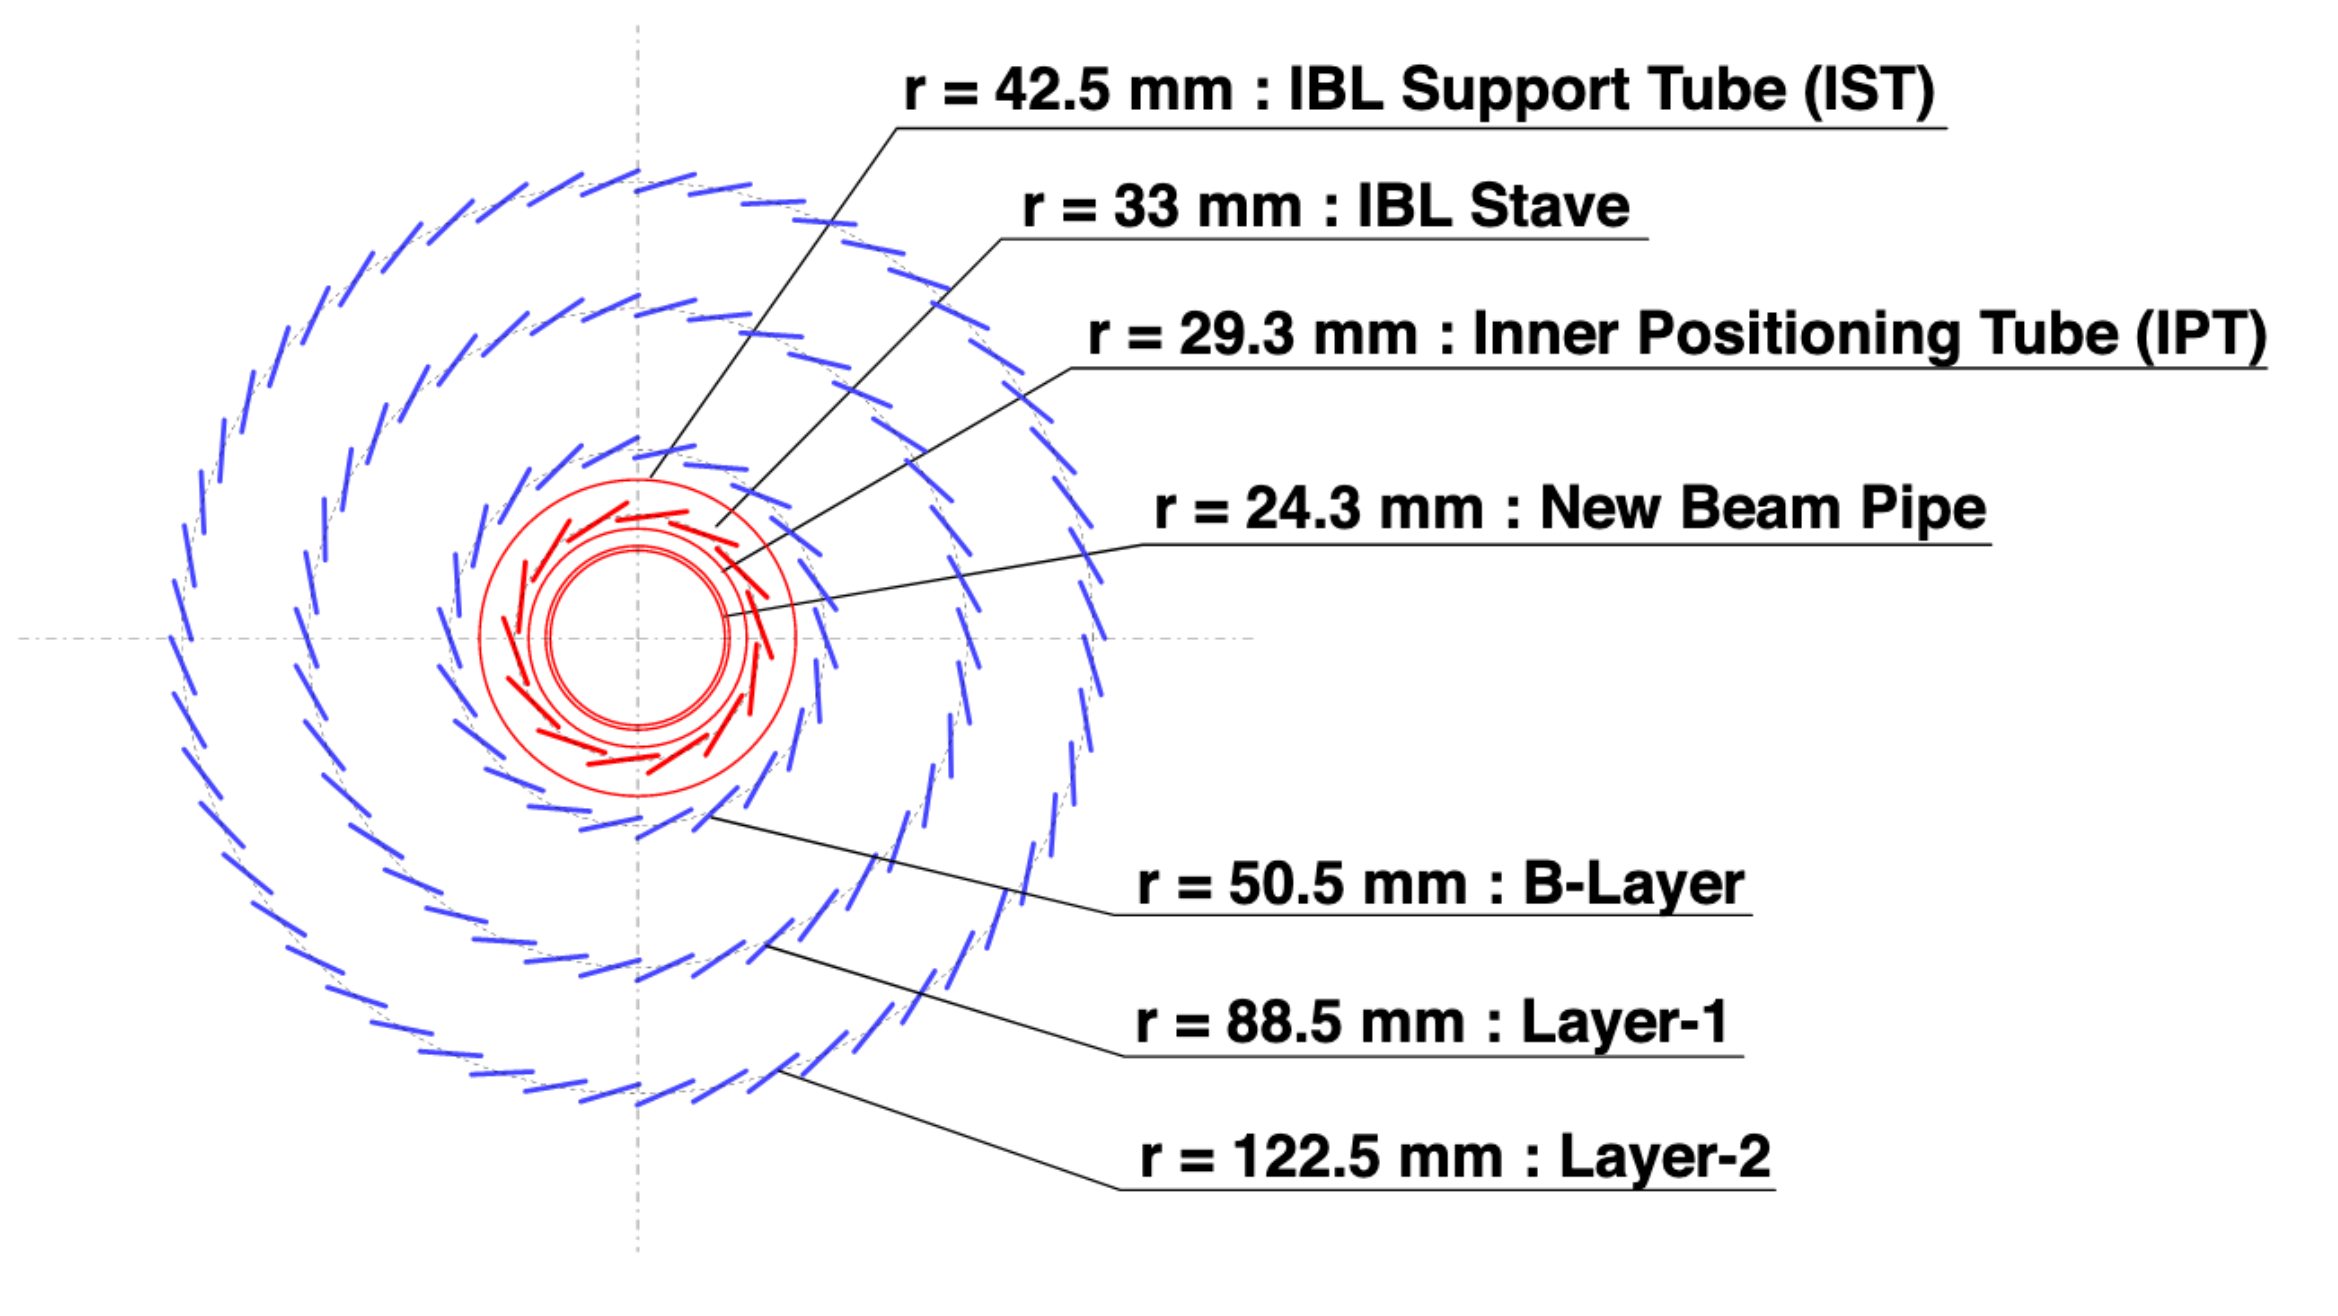
\includegraphics[width=0.75\textwidth]{pixel_ibl_cross_section}
	\caption{Radial placement of concentric pixel barrels, beam pipe, and carbon-fiber support cylinders (IST, IPT). \cite{Pernegger:1985432} }
	\label{fig:pixel_ibl_cross_section}
\end{figure}

\subsubsection{Semiconductor Tracker (SCT)}
The Semiconductor Tracker (SCT) is a silicon microstrip detector with 4088 modules arranged in four concentric barrels (2112 modules) and two endcaps (988 modules per endcap) of nine disks each.
The use of strips with dimension $63.56 \times 63.96$mm$^2$ instead of pixels is required due to the much larger coverage area (63 $\mathrm{m}^2$ vs. 1.7 $\mathrm{m}^2$) of the SCT when compared compared to the Pixel detector.
The silicon-strip detector technology further differs from pixels by requiring the combination of two measurements from separate strips aligned at stereo angles for each particle position measurement.
The SCT typically provides eight strip measurements (four position measurements) for each particle, with an intrinsic resolution of $17 \mu$m perpendicular to the strips in the $R-\phi$ plane (barrel) and 580 $\mu$m parallel to the beam in $z$ (barrel) and $R$ (end-cap).

\subsubsection{Transition Radiation Tracker (TRT)} 
The TRT detector is composed of carbon fiber reinforced Kapton drift tubes called ``straws'' with diameter of 4mm.
Inside of the straws reside 31 $\mu$m diameter gold-plated tungsten wires.
These tubes are interleaved with polypropyline or polyethylene fibers, which gives rise to so-called \textit{transition radiation} of the particles as they pass through alternating materials with different refractive indices.
Since transition radiation is more prominent in high-momentum, low-mass particles \cite{Andronic_2012}, this property underlies the primary use of the TRT in ATLAS: electron identification.

\subsection{Calorimeters}
\label{sec:calorimeters}

The calorimeter system measures particle energy and is located directly outside the solenoidal magnet surrounding the ID (Fig.~\ref{fig:calorimeter}).
The ATLAS calorimeter system is designed to fully absorb both charged and neutral particles\footnote{There are a few exceptions to this: muons, neutrinos, and extremely high energy particles that may ``punch through''.} such that they deposit their full energy into the calorimeter detector material.
Each separate ATLAS calorimeter technology provides granular coverage segmented in both $\eta$ and $\phi$.
Though they can provide some information about the direction of particles, the $\eta-\phi$ granularity of the calorimeter does not compare to that of the ID.

The ATLAS calorimeter system is composed of two types of calorimeters: electromagnetic and hadronic.
Both are sampling calorimeters which use alternating layers of active sampling material and inactive absorbing material.
When high energy particles interact with the dense absorbing layers, a shower of lower energy particles is created which interacts with the adjacent sampling material.
This results in a signal (electric current) proportional to the initial energy, which is then summed across all layers of the calorimeter system to measure the total energy of the particle.
The shape of the shower can also be determined by comparing the energy deposited in each layer, which results in some of the most useful particle identification information for ATLAS event reconstruction.
\znote{briefly explain why shower shape is useful}

\begin{figure}
	\centering
	\includegraphics[width=0.75\textwidth]{calorimeters}
	\caption{The ATLAS calorimeter system. The Inner Detector (visible, but greyed out) is enclosed by the Calorimeter system. © 2014 CERN.}
	\label{fig:calorimeter}
\end{figure}

\subsubsection{Electomagnetic Calorimeters}
The Electromagnetic (EM) calorimeter is the innermost layer of the calorimeter system and used for measuring the energy of electrons and photons.
It consists of a high-granularity lead-liquid argon (LAr) EM sampling calorimeter which covers the $|\eta| < 3.2$ region.
The energy deposits in the EM calorimeter primarily result from the charged particles in jets, bremsstrahlung radiation produced by electrons, and pair-produced electrons resulting from photons interactions within the calorimeter material.

The EM calorimeter is divided into a Barrel part (EMB) covering $|\eta| < 1.475$ and two End-Caps (EMEC) covering $1.375 < |\eta|\ < 3.2$.
Three separate cryostats are installed to to keep the liquid argon below its boiling point, and the services that compose the End-Cap cryostat necessitate a loss of EM calorimeter coverage in the $1.37 < |\eta|\ < 1.52$ region.
The EMB has three layers, each with slightly different purpose and segmentation granularity, as shown in Fig.~\ref{fig:em_calo_segment}.
The first layer is composed of narrow (in $\eta$) strips which provide precise measurements during the initial showering process.
The second layer is composed of square cells and is designed to fully capture moderate energy $(E < 50 \ \mathrm{GeV})$ photons and electrons.
The final layer of the EMB is less granular and meant to provide additional information about the longitudinal shower development for higher energy photons and electrons.
The EMEC follows the EMB segmentation design up until the end of tracking acceptance $(|\eta| < 2.5)$, after which it becomes coarser-grained with only two sampling layers.
\znote{define X0}

\begin{figure}
	\centering
	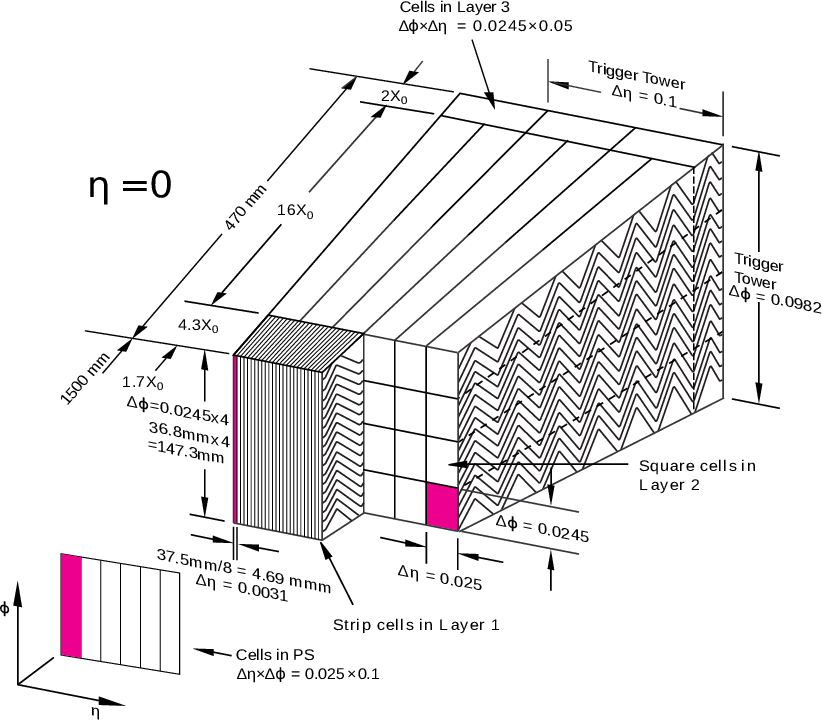
\includegraphics[width=0.75\textwidth]{em_calo_segment}
	\caption{Sketch of the ATLAS EM barrel calorimeter segmentation around $|\eta| = 0$. 
	The $X_0$ quantity is known as the \textit{radiation length} and quantifies the rate of energy loss with respect to traversed distance as a particle passes through a specific material.
	ATLAS Experiment © 2018 CERN.}
	\label{fig:em_calo_segment}
\end{figure}

\subsubsection{Hadronic Calorimeters}
The hadronic calorimeters are composed of two different technologies in different $|\eta|$ regions of the detector.
In the barrel region $(|\eta| < 1.7)$ resides the Tile Calorimeter composed of alternating layers of plastic active scintillator tiles and steel absorbing plates.
Like the EM calorimeter, particle showers are induced by the absorbing layer and particle showers are produced.
Unlike the EM calorimeter, strong force interactions play a role in addition to the electromagnetic interactions, resulting in the presence of hadrons in the showers.
When these hadrons pass through the plastic scintillator material, photons are emitted and detected by photomultipler tubes (PMTs) in order to produce the electrical signals which are then recorded and converted to an energy measurement.
The tile calorimeter is composed of three sections: one central barrel section $(|\eta| < 1.0)$ and two extended barrels sections $(0.8 < |\eta| < 1.7)$.

The Hadronic End-Cap (HEC) calorimeter provides hadronic energy measurements in the forward $(1.5 < |\eta| < 3.2)$ region.
Like the EM calorimeter it uses liquid argon as the active material, but copper plates as the absorbing material.
Each wheel of the HEC system is composed of two longitudinal layers, both located directly behind the end-cap cryostats.
\znote{for each calorimeter section, add granularity and dimensions from Tim Bristow thesis}

\subsubsection{Forward Calorimeter}
The forward region $(3.1 < |\eta|\ < 4.9)$ is covered by the Forward Calorimeter (FCal) which measures both electromagnetic and hadronic energy.
The FCal is composed of three concentric cylindrical modules which are themselves composed of a series of rods and tubes, where liquid argon fills the gaps between the rod and tubes as the active medium.
The first modules (closest to the beam line) use copper as an absorber and performs the electromagnetic energy measurement, while the second and third modules use tungsten as the absorber and perform the hadronic energy measurement.

\subsubsection{Calorimeter Resolution}
The calorimeter energy resolution can be generically parameterized as
\begin{equation}
    \frac{\sigma(E)}{E} = \frac{a}{\sqrt{E}} \oplus \frac{b}{E} \oplus c
    \label{eqn:calo_res}
\end{equation}
where $a$ is a stochastic/sampling term representing an intrinsic resolution limit due to particle fluctuations within the shower, $b$ is a noise term determined primarily by electronics noise and pileup, and $c$ is a constant term which dominates at high incident particle energy which is due to non-linearities in calorimeter response caused by inhomogeneity in detector materials, leakage due to un-absorbed particles from the shower, and calibration imperfections.
Each of these quantities $a$, $b$, and $c$ depend on the specific calorimeter detector technology under consideration.
The $\oplus$ operator denotes that each contributing term is summed in quadrature to estimate the final resolution.

The $a$ and $c$ quantities have been carefully measured for the ATLAS calorimeters \cite{Aharrouche_2006, Strizenec:2009zz, Cojocaru:2004jk, Adragna:2009zz} and are summarized in Table~\ref{tab:calo_res}.
The degradation of performance when moving towards higher values of $|\eta|$ is due primarily to the increased presence of pileup in these more forward regions closer to the beam line.
\znote{make sure pileup is defined somewhere previously}
The electronics/pileup noise ($b$) for each type of calorimeter is shown in Fig.~\ref{fig:calo_noise}.
Increased noise is acceptable in the more forward regions because the higher (on average) incident particle energy there diminishes the effect of the first two terms in Eq. \ref{eqn:calo_res}.

\begin{table}
\centering
\begin{tabular}{|c|c|c|} 
\hline
Region & $a\ [\%]$ & $c\ [\%]$ \\
\hline\hline
EM Barrel & 10.1 $\pm$ 0.1 & 0.17 $\pm$ 0.04 \\
\hline
EM End-Cap & 13.5 $\pm$ 0.5 & 0.7 $\pm$ 0.1 \\
\hline
EM Forward & 29.3 $\pm$ 0.7 & 3.0 $\pm$ 0.1 \\
\hline
Hadronic Barrel & 52.9 $\pm$ 0.9 & 5.7 $\pm$ 0.2 \\
\hline
Hadronic End-Cap & 88.0 $\pm$ 5.0 & 6.8 $\pm$ 0.4 \\
\hline
Hadronic Forward & 98.5 $\pm$ 4.0 & 6.4 $\pm$ 0.04 \\
\hline
\end{tabular}
\caption{
    Measured test beam resolution parameters for the ATLAS calorimeters.
    Each measurement is performed at specific impact points for each separate region: $0 < |\eta| < 0.7$ for the Barrel, $|\eta| = 2.8$ for the End-Caps and $|\eta| = 3.65$ for the Forward region.
}
\label{tab:calo_res}
\end{table}

\begin{figure}
	\centering
	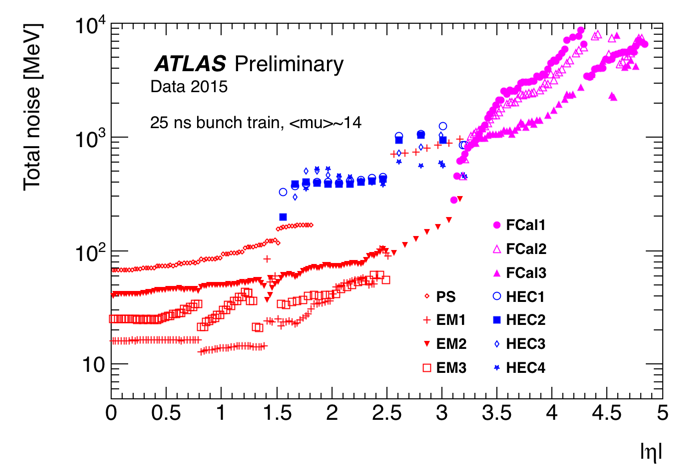
\includegraphics[width=0.75\textwidth]{calo_electronics_noise}
	\caption{Total electronics/pileup noise vs. $|\eta$| at the electron scale, measured in data with 25ns bunch spacing and $\langle \mu \rangle = 14$. ATLAS Experiment © 2015 CERN.}
	\label{fig:calo_noise}
\end{figure}

\subsection{Muon Spectrometer}
\label{sec:muon_spectrometer}
Muons are unique among the common Standard Model $p$-$p$ collision products by virtue of their long lifetime $(2.2 \mu s)$, weakly interacting nature, high production momentum and high mass $(\approx 200 \times m_e)$.
Due to these properties, muons pass through the ATLAS calorimeters without depositing a significant portion of their energy and leave only a weak ionization trail behind.
This necessitates the existence of the final outermost layer of the ATLAS detector: the Muon Spectrometer (MS) \cite{CERN-LHCC-97-022}, shown in Figure~\ref{fig:muon_spectrometer_cutout}.

\begin{figure}
	\centering
	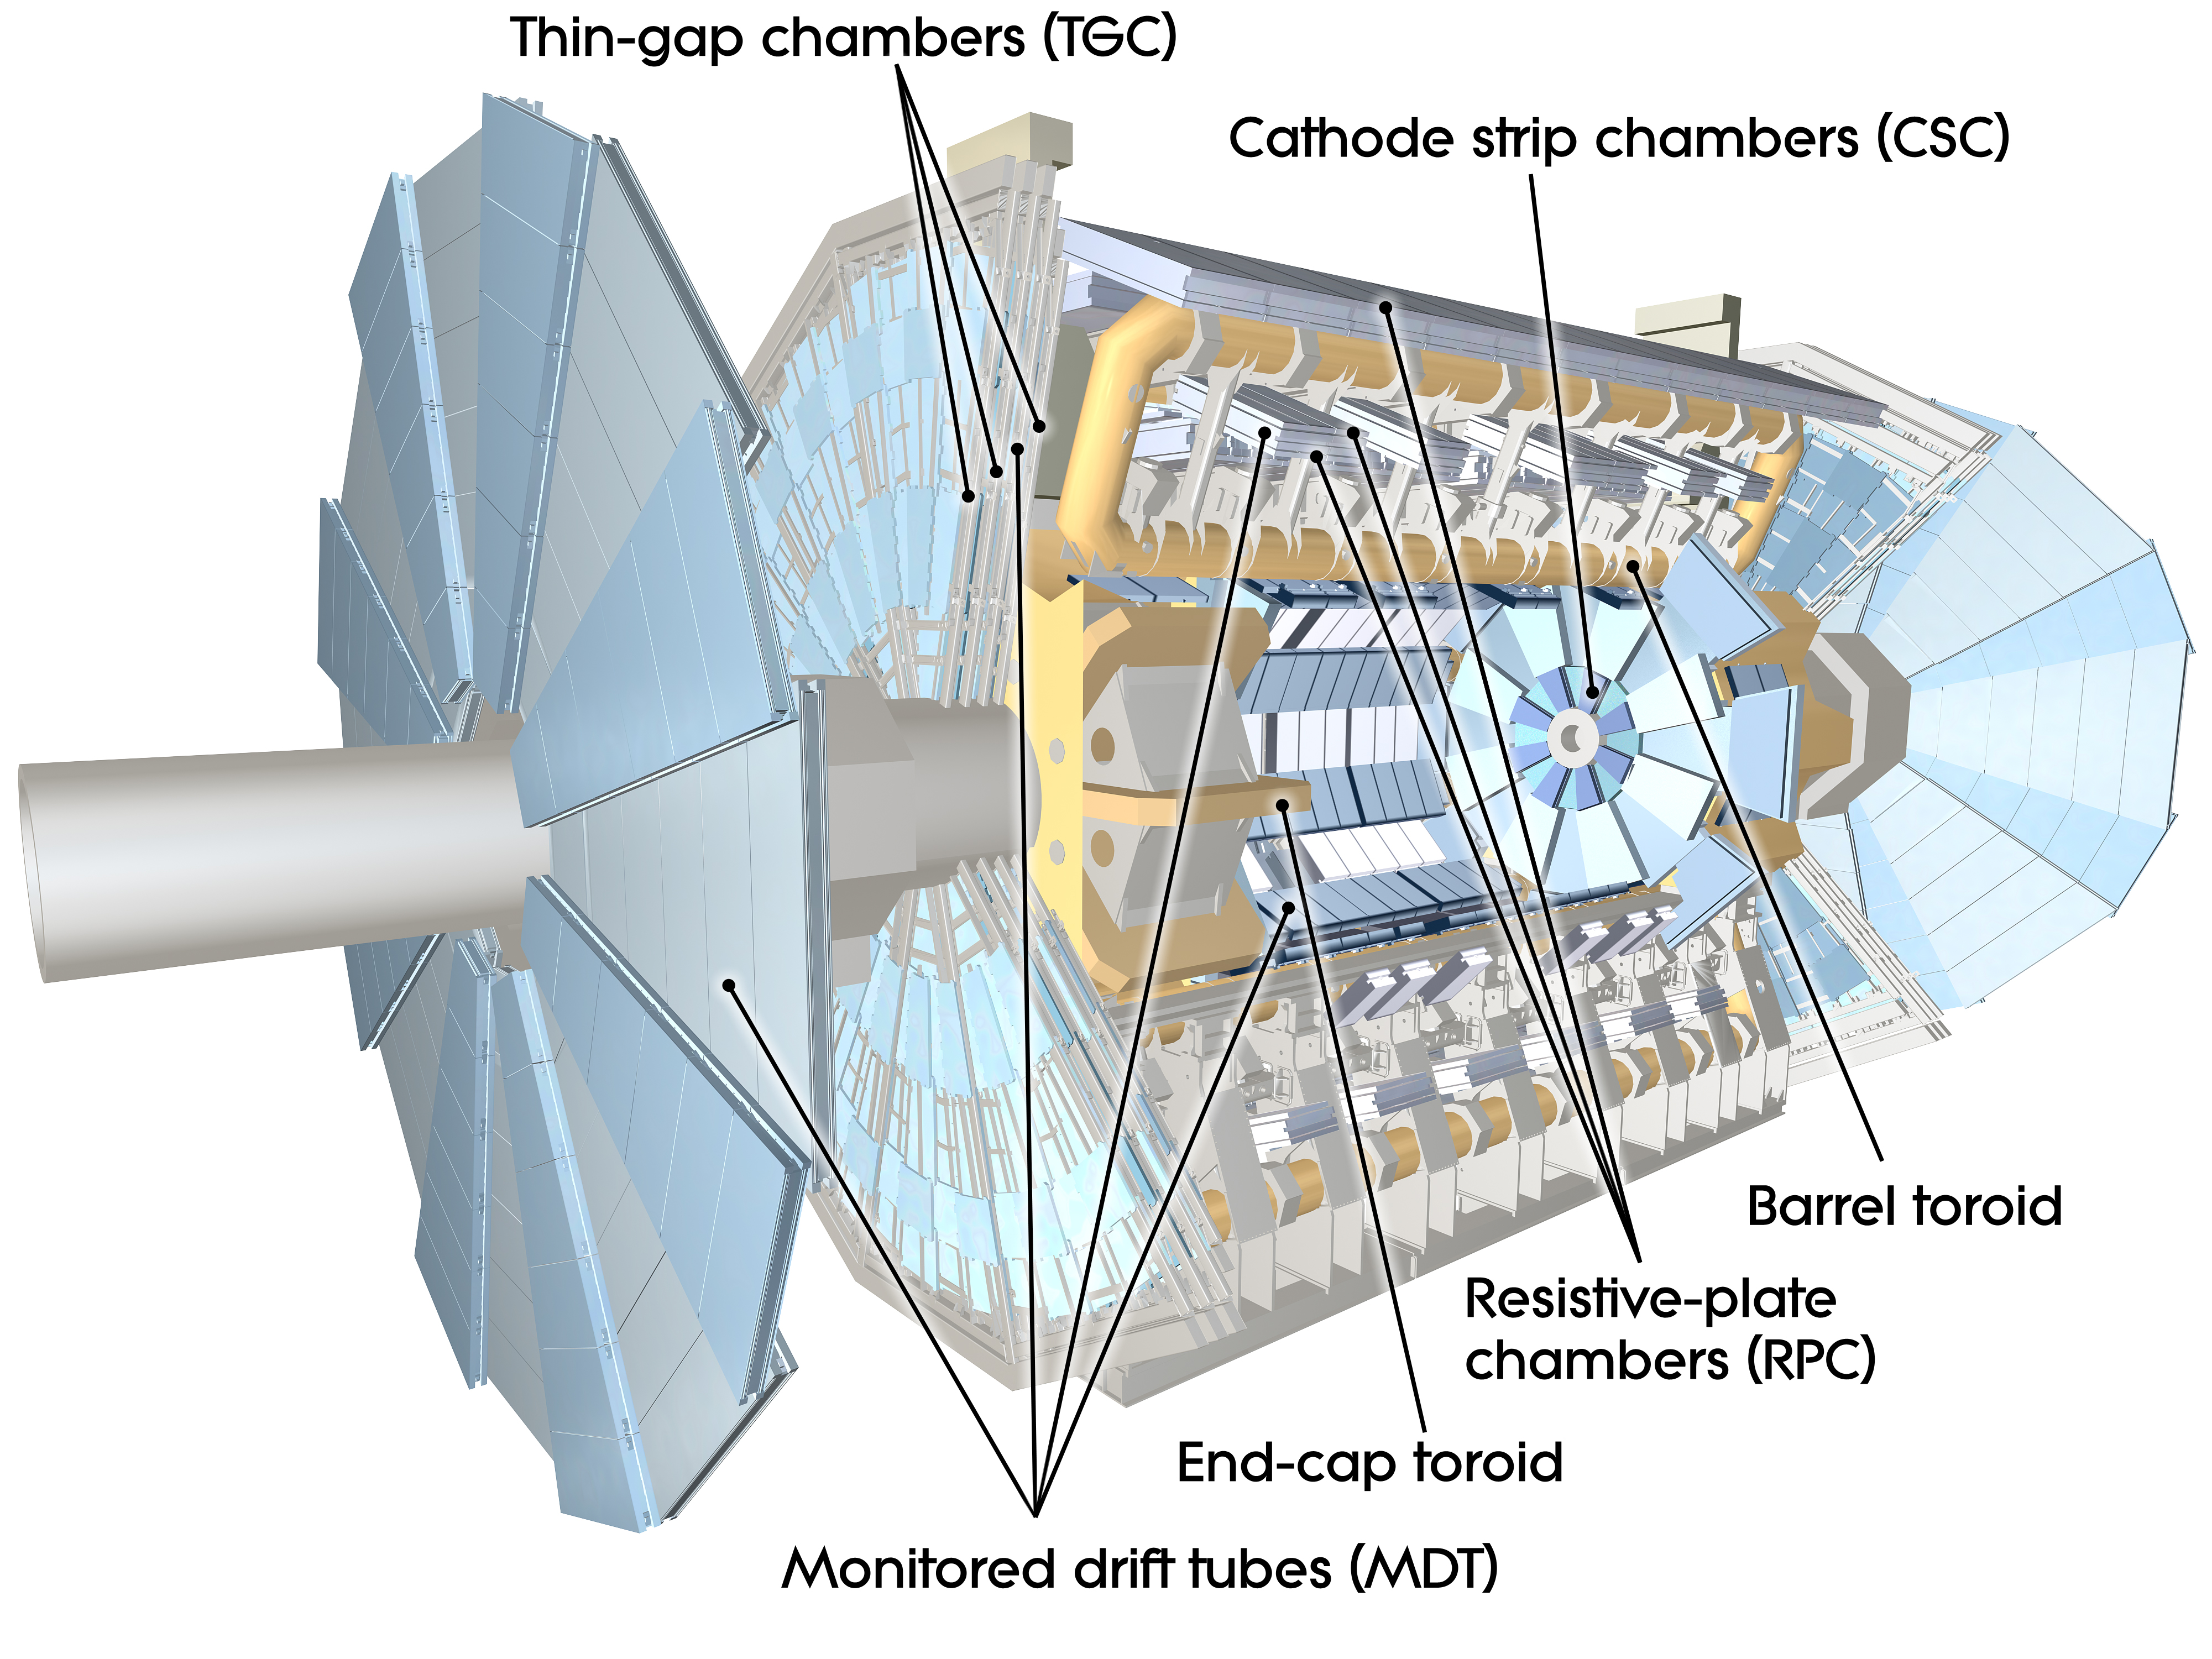
\includegraphics[width=0.75\textwidth]{muon_subsystem}
	\caption{ATLAS Experiment Muon Spectrometer. © 2014 CERN}
	\label{fig:muon_spectrometer_cutout}
\end{figure}

The MS consists of three air-core superconducting toroidal magnet systems (see Fig.~\ref{fig:ATLAS_magnet_system}) and four separate types of tracking chambers covering a region of up to $|\eta| < 2.7$, extending from a radius of 4.25m to 11m.
The magnet system of the MS serves to bend the trajectories of muons in the $R-z$ plane.
The large barrel toroid magnet strength depends strongly on $\phi$ and is active for $|\eta| < 1.6$.
The two smaller end-cap magnets (1 T) are active in the range $1.6 < |\eta|\ < 2.7$.

\begin{figure}
	\centering
	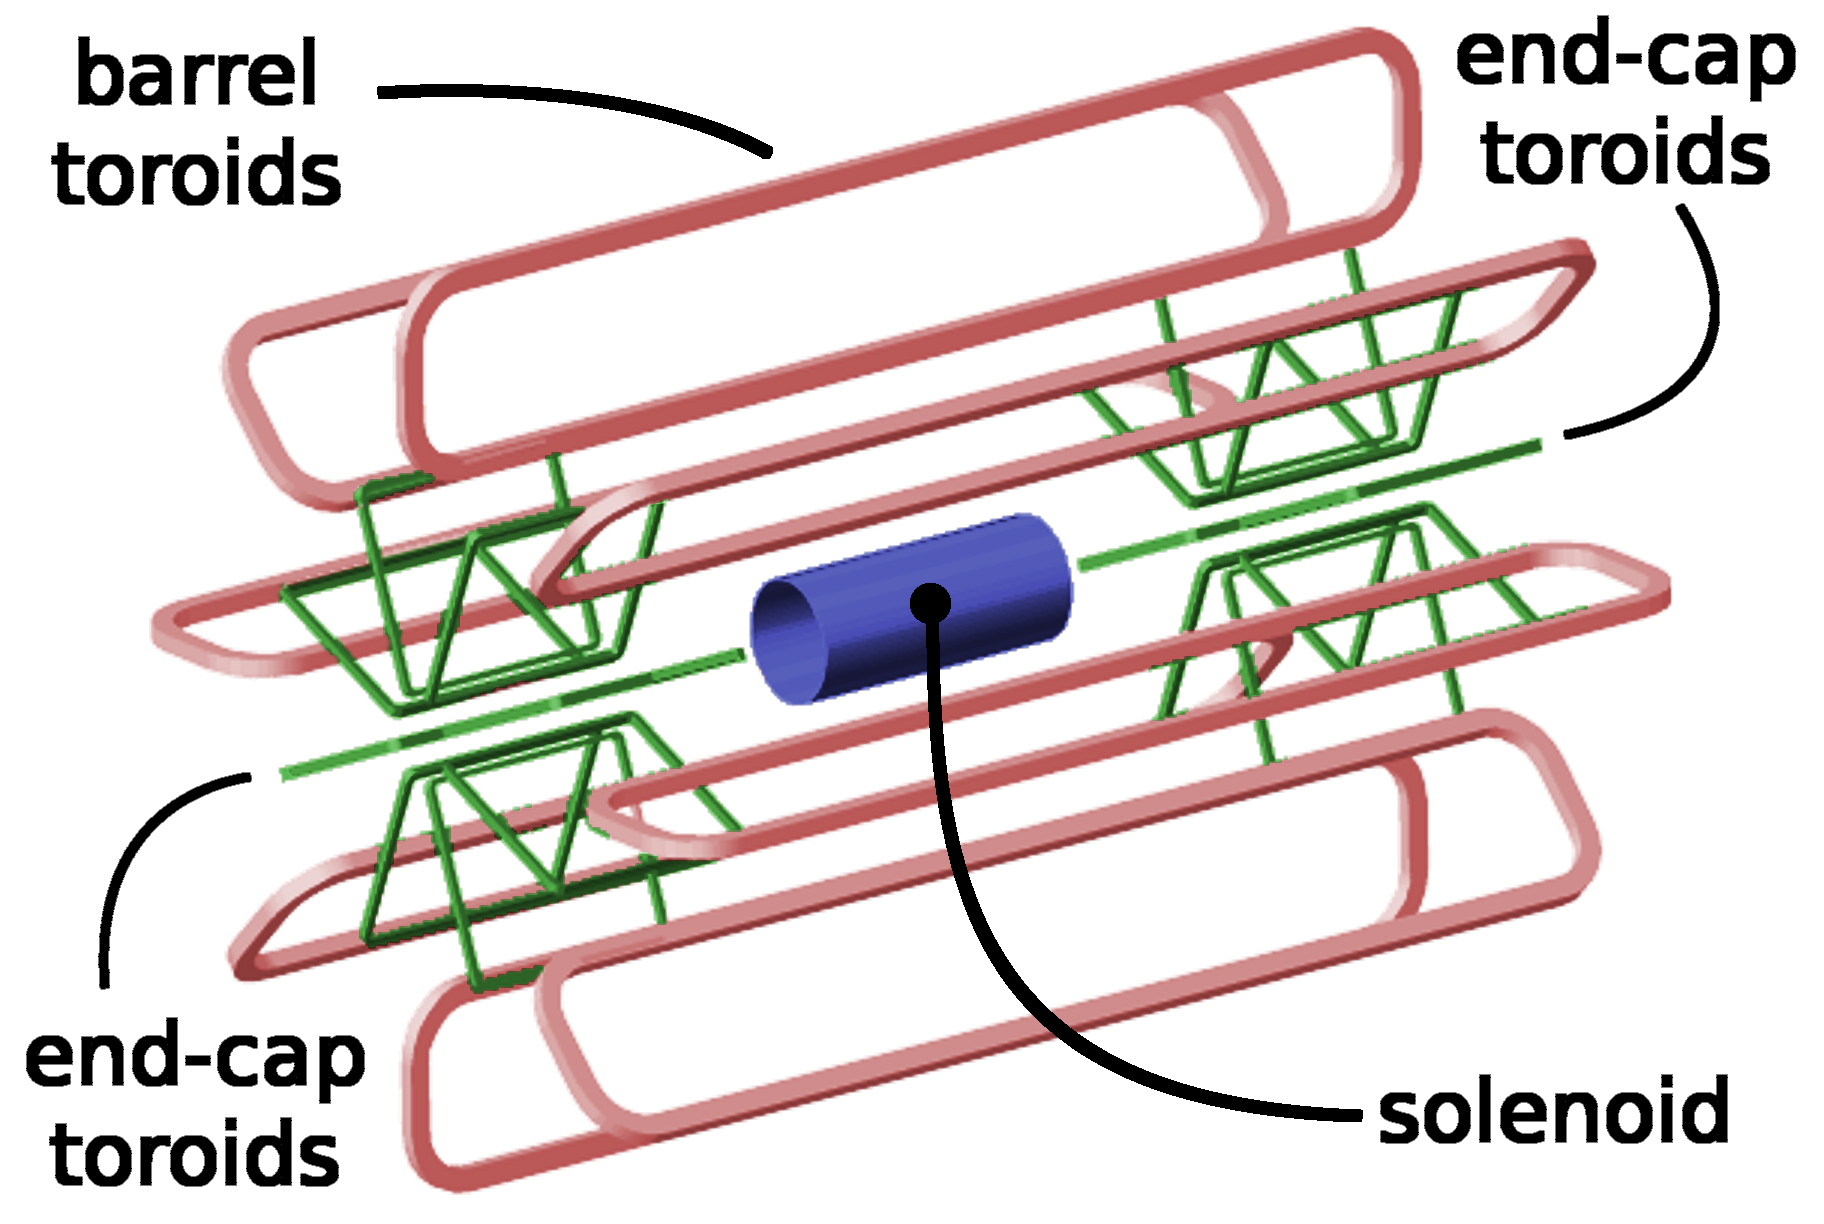
\includegraphics[width=0.6\textwidth]{magnet_systems}
	\caption{Illustration of the ATLAS magnet system. \cite{CERN-LHCC-97-018}
	The barrel region toroid magnet is shown in red and the two end-cap toroid magnets are shown in green. The inner solenoid is shown in blue, which is parallel to the beam pipe. © 2013 Jet Goodson}
	
	\label{fig:ATLAS_magnet_system}
\end{figure}

The MS is composed of several different types of detector technologies which are designed for two separate use-cases: (1) extending the precision tracking of each individual muon beyond the ID measurements and (2) fast readouts for the ATLAS trigger system.
Monitored Drift Tube Chambers (MDT) and Cathode Strip Chambers (CSC) are used for the high precision tracking measurements, while Resistive Plate Chambers (RPC) and Thin Gap Chambers (TGC) are less precise but provide a much faster readout, on the scale of nanoseconds, for the trigger system.
A cross section of the muon spectrometer highlighting the various sub-components is shown in Figure~\ref{fig:muon_spectrometer_cross_section}.
The tracking coverage $(|\eta| < 2.7$) of the MS is more complete than the trigger coverage $(|\eta| < 2.4)$.
Like the other major ATLAS detector components, the MS is split into separate barrel $(|\eta| < 1.05)$ and endcap $(1.05 < |\eta| < 2.7)$ regions.

\begin{figure}
	\centering
	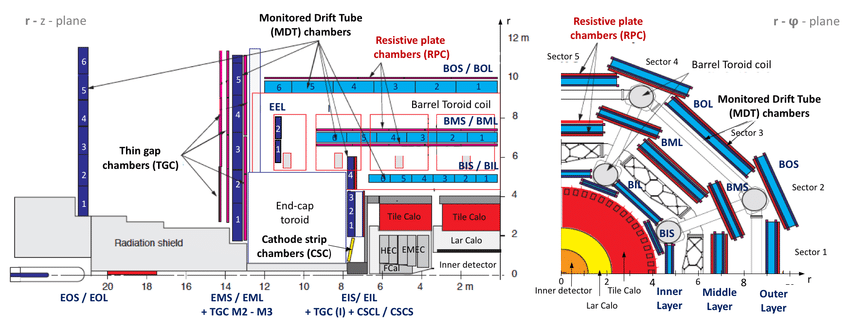
\includegraphics[width=0.9\textwidth]{muon_spectrometer_quadrant}
	\caption{
	 Cross-section of a quadrant of the ATLAS Muon Spectrometer \cite{kuger2017signal} in the $R-z$ plane (left) and the $R-\phi$ plane (right) comprising all detector modules. The naming of MDT chambers is based on their location in the barrel or end-cap (B,E), in the inner, middle, or outer layer (I, M, O) and in either the a large or a small sector (L,S).
	 © CERN
	}
	\label{fig:muon_spectrometer_cross_section}
\end{figure}

The MDT chambers are used for precision tracking of the $R-z$ plane curvature of muons.
They consist of 3-8 layers of 30mm diameter drift tubes between 0.8m and 6.5m long, filled with a mixture of $Ar/CO_2$ gas held at a pressure of three atmospheres.
Whenever the gas inside the drift tube is ionized by a passing muon, the resulting free electrons drift towards a 50 $\mu m$ W-Rh anode wire held at a voltage of 3kV in the center of the tube.
The precision tracking data from the barrel is measured by MDT chambers that cover the $|\eta| < 2$ range in the first layer, and up to $|\eta| < 2.7$ in the two outer layers.
There are three concentric barrel layers composed of MDT and RPC chambers at radii of 5m, 7.5m, and 10m.

The RPC chambers measure the non-bending coordinate ($\phi$) of muons.
They are composed of a set of parallel plate capacitors separated by a 2mm insulating space filled with a gas mixture of predominantly tetrafluoroethane ($C_2 H_2 F_4$). 
The plates have high resistance and are held at a constant high voltage, with metallic strips attached to their outer faces.
The fast response time of the RPC technology (1.5ns) makes it a prime candidate for the muon trigger system.
The RPC chambers are attached to the MDT chambers in the barrel and cover the central $|\eta| < 1.05$ region.

The CSC chambers replace the MDTs in the forward region of the first endcap layer of the MS in order to account for the high interaction rate in this region that would otherwise cause significantly degraded performance of the MDTs in this region ($2 < |\eta| < 2.7)$).
The CSC detector region is organized into two disks of sixteen chambers each.
Each CSC chamber consists of both a multi-wire proportional drift chamber as well as interleaved cathode strips placed parallel and perpendicular to the anode multi-wire layers.
The parallel cathode strips provide precision tracking measurement in the bending plane, while the perpendicular cathode strips provide measurements of $\phi$.

The TGC chambers are similar to the CSC chambers in design and consist of 50 $\mu m$ gold-plated tungsten anode wires, but with smaller gaps between electrodes for faster readouts.
They provide measurements of the $R$-$z$ and $\phi$ coordinates, covering the $1.0 < |\eta| < 2.4$ region.


% \subsection{Forward Detectors}
% The ATLAS experiment has additional detectors situated far away (20+ meters) from the interaction point which each serve a unique, specialized purpose.
% 
\subsection{Trigger and DAQ}
The LHC currently operates at a collision rate of 40 MHz.
Given that each event requires approximately 1.5 MB of disk storage, it is impractical to attempt to record every collision event observed by the ATLAS detector.
Not only would this require a bandwidth of $> 60$ TB/s, but only a small fraction of events are of interest to current HEP research efforts.
For this reason the trigger system \cite{Ruiz-Martinez:2133909} is used to reduce the recorded event rate to a more manageable level of approximately 1-2 kHz, which reduces the bandwidth requirement to 1~GB/s or less.
The trigger system operates in real-time at both hardware and software levels and ensures only events of interest to ongoing research are recorded by the ATLAS data acquisition system (DAQ).
For Run-2 ATLAS uses a two-tier trigger system: a hardware-based ``level-1'' (L1) trigger followed by a software based ``high-level'' (HLT) trigger.
Each trigger in the chain significantly reduces the data rate.
Only the events selected by the HLT are actually stored for offline processing/analysis.
A schematic of the full ATLAS trigger/DAQ system is shown in Fig.~\ref{fig:trigger_system}.

\begin{figure}
	\centering
	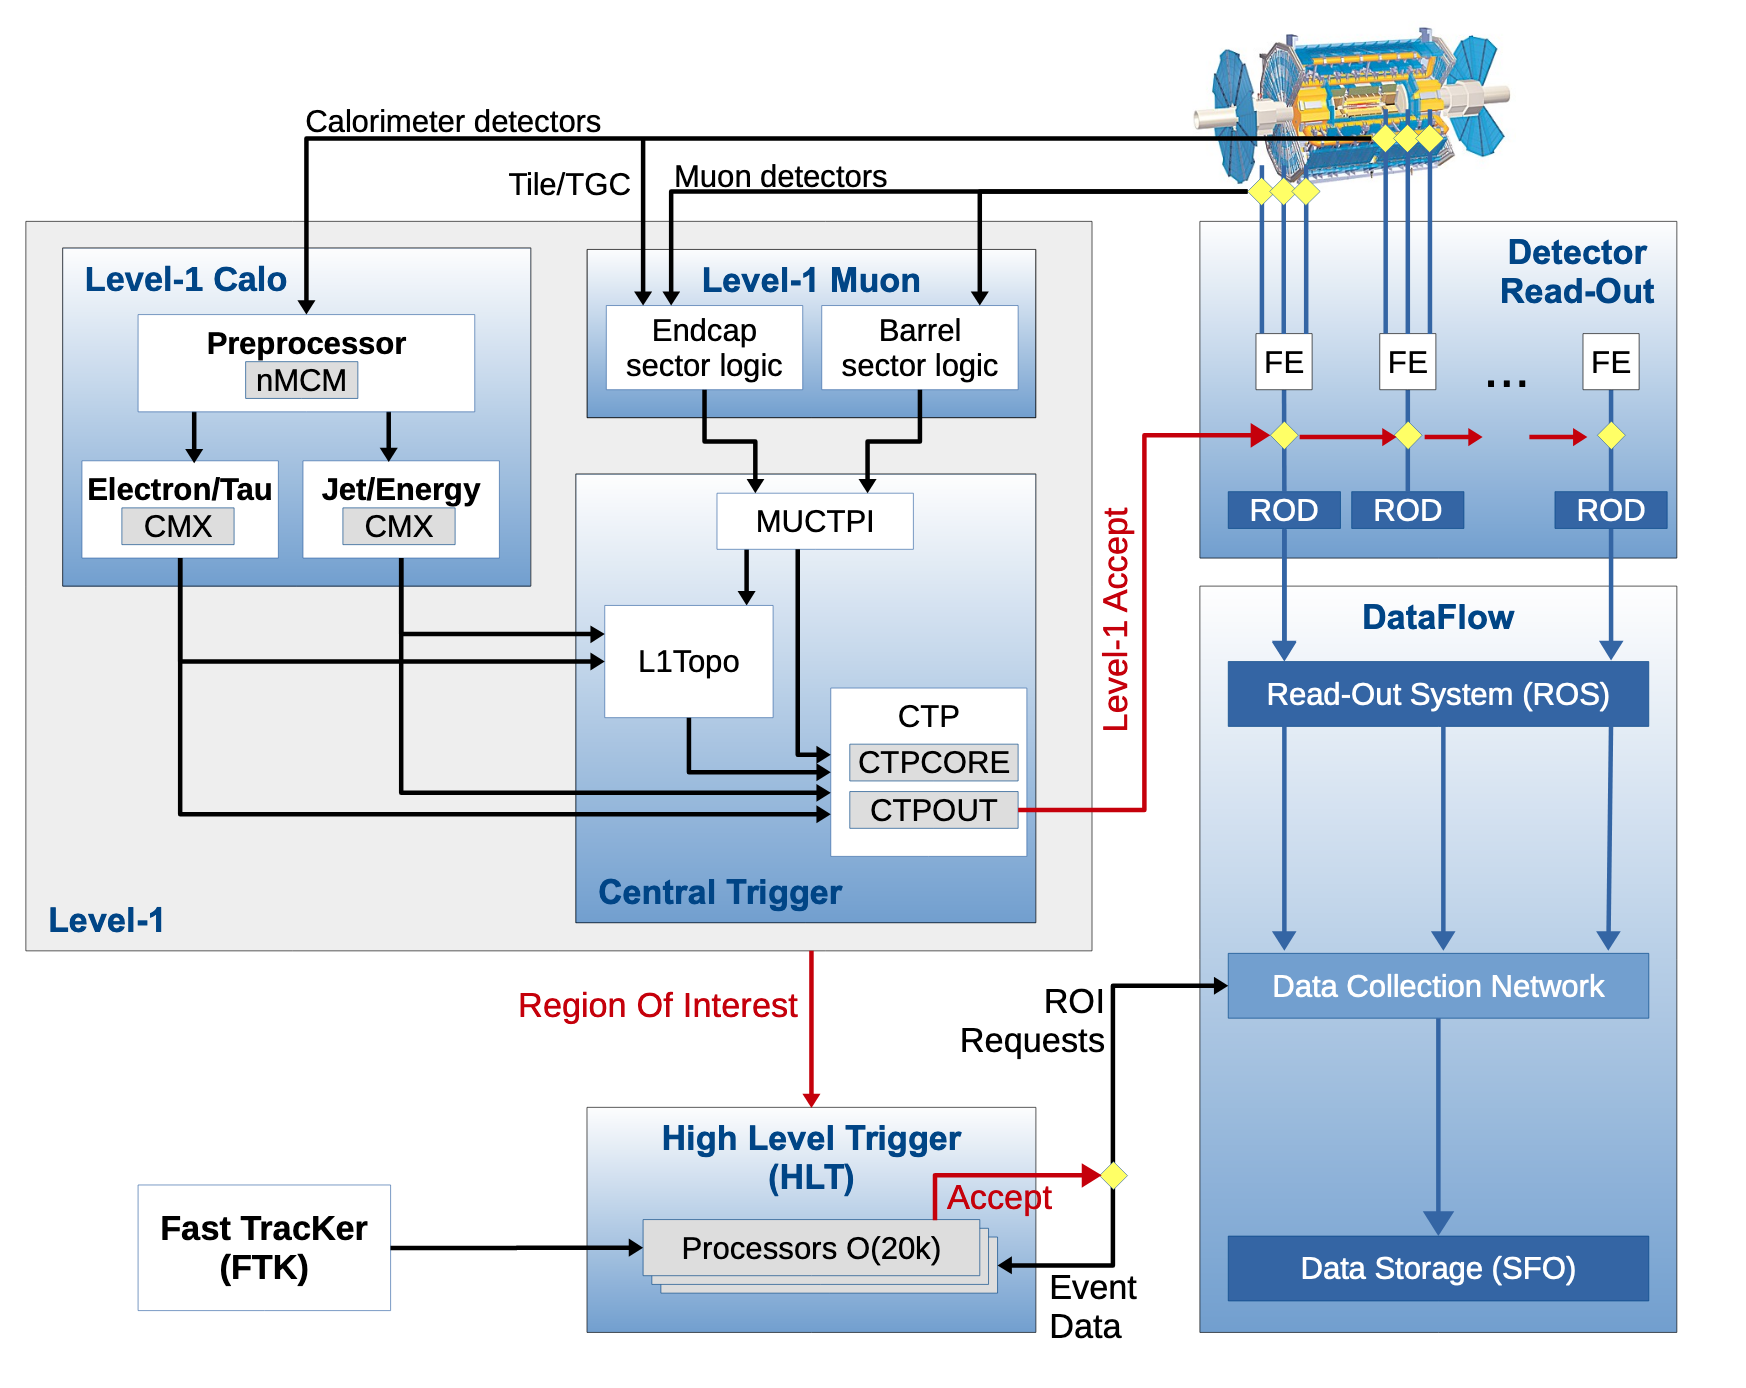
\includegraphics[width=0.8\textwidth]{atlas_trigger_system}
	\caption{Schematic layout of the ATLAS trigger and data acquisition system for Run-2. \cite{Ruiz-Martinez:2133909}}
	\label{fig:trigger_system}
\end{figure}

\subsubsection{Level 1 Trigger}
The L1 Trigger is a distributed electronics system located within the ATLAS detector which has sub-components that communicate with hardware from both the calorimeter (L1Calo) and muon spectrometer (L1Muon).
The L1Muon trigger processor interfaces directly with the dedicated muon trigger chamber hardware described in Section~\ref{sec:muon_spectrometer}.
The L1Calo trigger processor, on the other hand, relies on a form of modified calorimeter output called \textit{calorimeter trigger towers}.
These trigger towers consist of energy and timing sums for calorimeter regions with reduced granularity ($\Delta \eta \times \Delta \phi)$ ranging from $0.1 \times 0.1$ in the central region to $0.4 \times 0.4$ in the forward region.
A newer hardware-based L1 trigger labeled L1Topo analyzes kinematic/geometric relationships between different objects.
\znote{expand section about L1Topo}

The Central Trigger Processor (CTP) receives all the information in real-time from the L1Muon, L1Calo, and L1Topo processors.
The CTP first synchronizes the trigger inputs with the LHC collision clock in order to correctly associate each event with the correct bunch crossing.
All trigger inputs are then compared to different sets of trigger thresholds on the transverse momentum and various detector signatures, defined for each separate type of physics being targeted by ATLAS.
The choice of trigger thresholds is ultimately determined by the maximum allowed L1 output rate of 100 KHz, which represents a factor of 400 reduction from the 40 MHz event rate at the LHC.
If any set of trigger thresholds are passed, the CTP flags the event as accepted and notifies all sub-detectors.
Upon receiving this ``L1 Accept'' (L1A) notification, all the data from each sub-detector is read out and propagated to the next step in the trigger process: the High Level Trigger.
\znote{mention ROIs}

\subsubsection{High Level Trigger}
The HLT is a software based trigger that refines set of events passing the L1 trigger using the full information available from the ATLAS detector, as opposed to the low granularity data used by the L1 trigger.
For example, the HLT uses tracking information from the ID to locate the primary vertex (PV) \znote{cite vertexing section} and various particle candidates.
The HLT reduces the data rate from 100 KHz to approximately 1 KHz.
Since the HLT is software based it is limited primarily by the CPU processing time and must be highly optimized to process each event in approximately 0.1 - 1.0 seconds.
An example of such an optimization is that track reconstruction \znote{cite tracking section} is only performed within ROIs defined by the L1 trigger.

\subsection{Computing}
The raw data for all events passing the ATLAS trigger system is sent to the CERN Data Center where the process of archiving, distributing, processing and analyzing begins.
However, this is only the starting point of an international network of LHC computing resources \cite{Bird:1447125} known as the Worldwide LHC Computing Grid (WLCG) or simply ``the grid''.
The WLCG is a layered system made up of three separate ``tiers'' as shown in Fig.~\ref{fig:wlcg_tiers}.

\begin{figure}
	\centering
	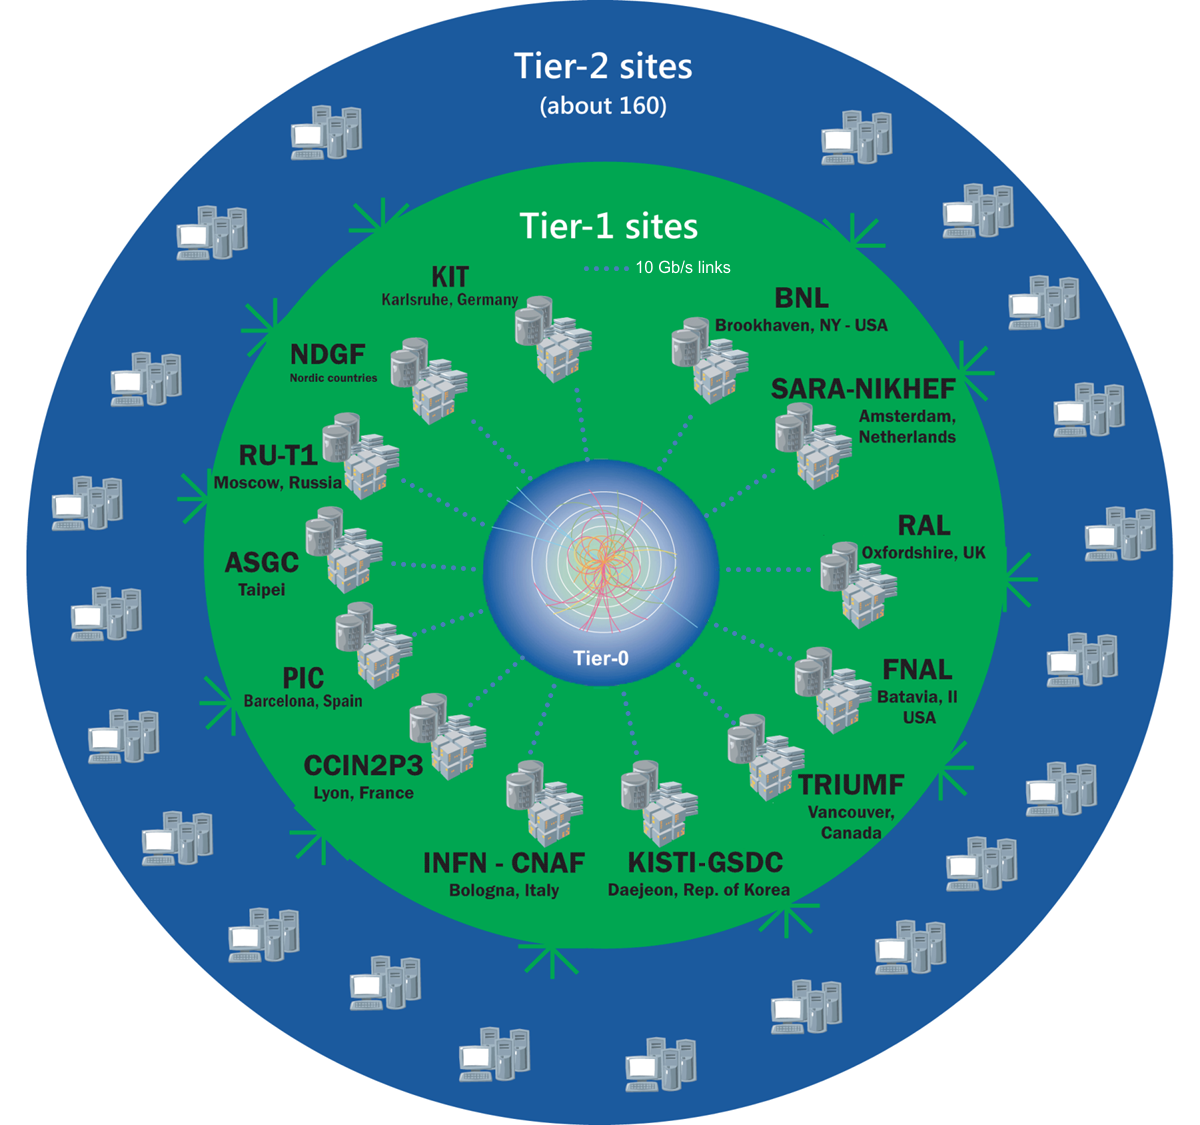
\includegraphics[width=0.65\textwidth]{wlcg_tiers}
	\caption{Schematic diagram of the Worldwide LHC Computing Grid tier system. © 2020 CERN.}
	\label{fig:wlcg_tiers}
\end{figure}

The CERN Data Center (\textbf{Tier-0}) provides around 20\% of the total compute capacity of the LHC, with the other 80\% coming from institutions around the world.
The next layer of support (\textbf{Tier-1}) is composed of thirteen large computing centers with round-the-clock support and massive storage capacity.
They are responsible for large-scale reprocessing, storage and safe-keeping of a significant proportion of raw and reconstructed data from the LHC.
Furthermore, Tier-1 centers share these resources with the next link in the chain (Tier-2).
Tier-1 centers are typically national laboratories such as BNL, INFN, and TRIUMF.

The next link in the chain (\textbf{Tier-2}) is composed primarily of universities and other scientific institutions which possess enough storage and computing power for a combination of analysis tasks, simulated event production and reconstruction.
Individual scientists connect to the grid via the last tier (\textbf{Tier-3}) which consists of local computing resources such as small local clusters belonging to individual Physics departments or even individual PCs.
